\documentclass[12pt]{report}
\usepackage{graphicx} % Required for inserting images
\usepackage{xcolor}
\usepackage[a4paper,left=1in,right=0.75in,top=0.75in,bottom=0.75in]{geometry}
\usepackage{times}
\usepackage{hyperref}
\usepackage{amsmath}
\usepackage{subfigure}
\usepackage{tikz}
\usepackage{titling}
\usepackage{longtable,booktabs,array}
\usepackage{multirow}
\usepackage{calc} % for calculating minipage widths
\usepackage{etoolbox}
\makeatletter
\patchcmd\longtable{\par}{\if@noskipsec\mbox{}\fi\par}{}{}
\makeatother

% paragraph indent
\usepackage{parskip}
\setlength{\parindent}{0em}
\setlength{\parskip}{1em}
\renewcommand{\baselinestretch}{1.25}

% reference list
\usepackage[
backend=biber,
style=alphabetic-verb,
sorting=ynt
]{biblatex}
\addbibresource{reference.bib}

% algorithm and procedure
\usepackage{algorithm}
\usepackage{algorithmic}
\newcommand\algorithmicprocedure{\textbf{procedure}}
\newcommand{\algorithmicendprocedure}{\algorithmicend\ \algorithmicprocedure}
\makeatletter
\newcommand\PROCEDURE[3][default]{%
  \ALC@it
  \algorithmicprocedure\ \textsc{#2}(#3)%
  \ALC@com{#1}%
  \begin{ALC@prc}%
}
\newcommand\ENDPROCEDURE{%
  \end{ALC@prc}%
  \ifthenelse{\boolean{ALC@noend}}{}{%
    \ALC@it\algorithmicendprocedure
  }%
}
\newenvironment{ALC@prc}{\begin{ALC@g}}{\end{ALC@g}}
\makeatother

\newcommand{\algorithmautorefname}{Algorithm}
\graphicspath{{./image/}}

\newcommand{\mynote}[2]{\fbox{\bfseries\sffamily\scriptsize{#1}} {\small\textsf{\emph{#2}}}}
\newcommand{\tb}[1]{\textcolor{red}{\mynote{boris}{#1}}}
\newcommand{\tudinh}[1]{\textcolor{orange}{\mynote{TU}{#1}}}
\newcommand{\son}[1]{\textcolor{blue}{\mynote{DX}{#1}}}
\newcommand{\hieplnc}[1]{\textcolor{brown}{\mynote{hieplnc}{#1}}}

\title{Regression methods for analysis of rice spectral reflectance data }
\author{PHAM Phan Bach}
\date{\today}

\begin{document}

%\maketitle
\begin{titlepage}
    \begin{tikzpicture}[remember picture,overlay,inner sep=0,outer sep=0]
     \draw[black!70!black,line width=1.5pt] ([xshift=-1.5cm,yshift=-2cm]current page.north east) coordinate (A)--([xshift=2cm,yshift=-2cm]current page.north west) coordinate(B)--([xshift=2cm,yshift=2cm]current page.south west) coordinate (C)--([xshift=-1.5cm,yshift=2cm]current page.south east) coordinate(D)--cycle;

   \end{tikzpicture}
    \begin{center}
    \MakeUppercase{\Large{{University of Science and Technology of Hanoi}}} \\ 
    \MakeUppercase{\Large{\textbf{Master's degree}}} \\ [1cm]
    
    \begin{figure}[ht!]
        \centering
        
\includegraphics[width=.5\textwidth, height=\textheight, keepaspectratio]{logos/usth-logo.png}
    \end{figure}
            
    \vspace {0.5cm}
    \Large{Research and Development} \\
    \MakeUppercase{\Huge{\textbf{Master thesis}}} \\ [1cm]
    \Large{by} \\
    \Large{\theauthor} \\
    \Large{M21.ICT.002} \\
    \Large{Information and Communication Technology} \\ [0.75cm]
    \Large{Title:} \\
    \huge{\textbf{Regression methods for analysis of \\ rice spectral reflectance data}} \\[0.75cm]
    \Large{Supervisors: Dr. TRAN Giang Son \\Lab name: USTH's ICT lab} \\ [1.5cm]
    
    \Large{\textbf{Hanoi. Oct 2024}}
    \end{center}
\end{titlepage}

% attestation
\chapter*{Attestation}
I hereby, \theauthor, certify that my thesis doesn’t contain plagiarism (copy/paste) from other sources.

\vspace{5mm}
\noindent%
In case of plagiarism in my thesis, I know the consequences and I understand that my thesis won’t be evaluated. In this case, my M2 internship will be noted as "fail". 

\vspace{1cm}
\noindent%
Sep, 10th, 2023 \\
Signature 

\vspace{2cm}
\noindent%
\theauthor

% ack
\chapter*{Acknowledgements}

\noindent%
My thesis would not be completed without the help of many people to whom I wish to express gratitude. 

First and foremost, I would like to express my gratitude to my supervisor Dr. TRAN Giang Son, for orginating the opportunity for my internship in ICT lab. His constructive instruction and feedback during both before and throughout the internship is indispensable for the project completion

\vspace{5mm}
\noindent%
In addition, I take this opportunity to especially thank Dr. NGHIEM Thu Phuong and MSc. LE Nhu Chu for their guidance and encouragement during my study time in ICTLab.

\vspace{5mm}
\noindent%
Thanks should also go to all my friends and colleague in ICT lab for their helpful discussions and assistance. 

\vspace{5mm}
\noindent%
Last but not least, I would also extend my deep appreciation to my family and friends for their continuous love, unwavering support throughout my life.


\noindent%
 \newline

% toc
\pagenumbering{gobble}

\tableofcontents
\clearpage
\thispagestyle{empty}

\addcontentsline{toc}{chapter}{\listfigurename}
\listoffigures
\clearpage

\addcontentsline{toc}{chapter}{\listtablename}
\listoftables
\clearpage

% \chapter*{Abstract}
% \addcontentsline{toc}{chapter}{Abstract}
% \input{abstract}
% \clearpage

% count from starting of contents
\newpage
\pagenumbering{arabic}
\setcounter{page}{1}

\chapter{Introduction} \label{chap:introduction}
\section{Context \& Motivation}

Rice is well known as an indispensable ingredient providing daily nourishment for more than half of the world's population.
With the upward trends of the world's population projections,
it has become more and more essential to not only maintain but also increase the rice yield efficiency.
The health of rice production has been proven to be linked directly to the amount of nutrients in the plants,
especially Chlorophyll (Chlo), Phosphorus(P), and Potassium (K).
A lower level of concentration means a diminished yield.
A sufficient amount of Nitrogen will improve plant size, spikelet, panicle health, and yields.
Phosphorus affects the rice's flower blooming cycle, helps root growth, and plants immunity against diseases and drought. \cite{hindersah2022rice}
Potassium increases rice's culm strength and prevents plants from topping on each other.
However, fertilizing crops excessively can lead to reducing the branch strength and attracting unwanted
vermin, fungi, and other foreign organisms.
The appearance of leaves, including their color, shape, and sheath, provides valuable information
about a plant's nutrient and health status,
which is closely tied to its nutritional content.
The measurement of the chemical components present in a plant can be determined through its leaves and canopy's spectral reflectance signature.

While analyzing spectral reflectance gives the most accurate result,
this method can only be done on a small scale due to its high-cost, time-consuming, labor-intensive process.
The fertilization also needs to be carried out in a timely manner during the plant growth stage.
Remote sensing is one of the more practical approaches for monitoring hundreds of hectares of rice fields.
It can be swiftly deployed over larger areas with minimum impact on the crops.
The plant's nutrition content can be analyzed through hyper-spectral imaging techniques.
Drone armed with multi-spectral cameras with very high spatial resolution are flown over the fields
and gather images in hundreds of different bandwidths.
Scientists from many fields have been using these hyperspectral images to analyze many chemical components in crop leaves.
In spite of their usefulness, the task of processing the data and accuracy of crops determined nutrition values leaves a lot to be desired.


One of the more popular method is ultilising normalized difference vegetation index also known as NDVI. However, since it constists of 2 specified bandwidth red and infrared, there a thounsands of combination pairs. Therefore it is quite a challenges to maximize the method effectiveness. This is where we apply machine learning. Machine learning techniques if implemented properly, are regarded as a powerful for predicting agriculture indices using data obtained from specialised remote sensing machine\cite{behmann2015review}. They are capabled of autonomously solving nonlinear challenges using dataset combined from multiple variables, which resolves our labor problem. Their result when analyze with a large number of bandwidths and others spectral information have proven to be quite promissing \cite{van2014gaussian}. Machine learning can ultilise more informative features and generate a high-accuracy predicton modelling\cite{panda2010application}.

\section{Objectives}
The objective of this project is to find the best prediction result, along with it the pairs of NDVI's wavelegth correspondingly to the best models, First, we need to develop multiple model capable of identifying the concentrations of Phosphorus (P), potassium (K), and Chlorophyll-a based on reflectance data collected from replicates and their sub-replicates. Afterwards, these regression technique is extensively examined and analysed through multiple different bandwidth. In summary, we aim to comprehensively assess the accuracy and precision of our models and spectral band, providing valuable insights into their performance and suitability for its practical applications.

% Fix these
\section{Related Work}
During the time working on this study, multiple documents with similar topics and challenges was used as reference documents. In the research “Spectral Reflectance Characteristics and Chlorophyll Content Estimation Model of Quercus aquifolioides Leaves at Different Altitudes in Seijila Mountain” \cite{zhu2020spectral}, by using a dataset of 60 samples  of spectral parameters explored regression models to predict Chlorophyll content. Their analysis contains 9 different spectral characteristics of plants as predictor variables, with Chlorophyll content serving as the response variable. They applied univariate regression techniques including index, linear, and quadratic polynomial models, to control accurate estimation models. As for the result, the R-squared for the RGP model seems to be the greatest one with remarkable values of 0.8523.
Another work that was used as reference is the study of “Predicting Nitrogen Content in Rice Leaves Using Multi-Spectral Images with a Hybrid Radial Basis Function Neutral Network and Partial Least-Squares Regression” \cite{yu2018development} is the combination of Multi-Spectral Imagse, a Hybrid Radial Basis Function Neural Network, and Partial Least-Squares Regression. The evaluation metrics are MAE, MAPE, and RMSE (similar to MSE but different when RMSE is the square root of MSE). The most remarkable performance goes to the RBFNN model which is outstanding in both the growing and mature stages. During the growing stage, it achieves a MAPE of 0.5399, while with the mature stage, it records a MAPE of 0.1566. These results when compared with GRL seem to be surpassed when this model has the MAPE of 1.0545 with the growing stage and 0.7399 with the mature stage. Which also performs well is the GRM with 1.2395 of MAPE in the growing stage and 1.2272 in the mature stage. 

\section{Thesis organization}
The thesis is structured as follows:
\begin{itemize}
    \item Section 1: Introduction \& Objectives
    \item Section 2: Materials and methods
    \item Section 3: Result
    \item Section 4: Conclusion \& Future works
\end{itemize}


\chapter{Material \& Methodology} \label{chap:methodology}
\section{Material} \label{material}
The experiements is conducted in Lam Thao District, Phu Tho province, Vietnam. This part is favorable for its location within the Red River delta, under the influence of tropical weather and sustain 1720 mm of annual rainfall. It have been ultilised by local residents for cultivating rice for years. Our sample rice field is sepperated into 54 part of 100m2 square parcels. With the help of locals farmer, the parcels are fertilized into differents amounts of N, P, K which will cause variation in leaf's spectral reflectance. The farmers was also request for their expertises to take care of the rice field during its growth stages to minimize the crops harms because of water stress or diseases. In each divided parcels, the data is extracted 3 times using specialised machine for measuring spectral reflectance.

The data is captured into a folder with two types of files: a set of sed files and csv file. The sed files are taken from the specialised machine while contains a great deal of information, most of them are unnecessary for the project. Each row in the csv file is correspond to a sed file. For the information to be usable, both type of files need to be combined to a comprehensive and informative dataset 


\begin{figure}[h]
\centering
    \subfigure[]{\includegraphics[width=1\textwidth]{image/Ground_mesurement_20220519.png}}
\caption{The sample field with 54 rice parcels} \label{fig:rice-field}
\end{figure}
    
    

\paragraph{Structure of .sed files} 
Number of .sed files: 260 files.
\begin{itemize}
    \item Content in a .sed file:
    \item Version: 2.3 [1.2.6250C]
    \item File Name
    \item Instrument: PSR-2500-SN1726293 [2]
    \item Detectors: 512,0,256
    \item Measurement: REFLECTANCE
    \item Date
    \item Time
    \item Temperature (c) 
    \item Battery Voltage
    \item Averages: 10,10
    \item Integration: 10,30,20,30
    \item Dark Mode: AUTO, AUTO
    \item Foreotopic: LENS {RADIANCE}, LENS4 {RADIANCE}
    \item Radiometric Calibration: RADIANCE
    \item Units: W/m2 /sr/nm
    \item Wavelength Range: 350,2500
    \item Latitude
    \item Longtitude
    \item Altitude
    \item GPS Time
    \item Satellites
    \item Calibrated Reference Correction File: none
    \item Channels: 2151
    \item Columns [4]

\end{itemize}

Each file also contain 2151 data, corresponding to wavelength channel captured from 350-2500 
\begin{itemize}
    \item Wavelength (Wvl)
    \item Reference Radian (Rad. (Ref.))
    \item Target Radian (Rad. (Target.))
    \item Reflect (Reflect.)
\end{itemize}

\paragraph{Structure of csv files}
There are 61 replicates, with 171 data row
\begin{itemize}
    \item Latitude
    \item Longitude
    \item Replicate, Sub-replicate
    \item Concentration of P, K (mg/kg)
    \item Chlorophyll-a
\end{itemize}

\begin{table}[H]
    \centering
    \begin{tabular}{c c c c c c} 
        \hline
        \textbf{Nutrients } & \textbf{Sample} & \textbf{Mean} & \textbf{Min} & \textbf{Max} & \textbf{St. Deviation}  \\
        \hline
        Chlorophyll  & 171 & 41.84 & 33.0 & 48.6 & 3.10  \\
        P concentration & 171 & 4317.11 & 1124.0 & 7740.0 & 805.68  \\
        K concentration & 171 & 35975.34  & 12620.0 & 59730.0 & 10578.94  \\
        \hline
    \end{tabular}
    \caption{Table of Nutrients’ statistics description} \label{table:mem-page-to-mem-size}
\end{table}

\section{Methodology} \label{section:background}


In this section, several necessary knowledge is discussed before the reader could understand deeply on our work problem and solution.

\subsection{Spectral Reflectance}
% Challenge:
% It is difficult for the reader to understand about value of input.
% It is potential to bring back enrich information from the spectral reflectance.
% Objective:
% Defition, collective method, enriched information, useful of information.

% What is the spectral reflectance
The reflectance is the effectiveness in reflecting radio energy of a surface,
and different radio wavelength has different reflectance on the same surface.
By combining multiple wavelength reflectance,
we gain a spectral reflectance of the targeted surface.

% Characteristic of reflectance
It is a highlight that different material provides different reflectance spectrum
basing on the material physical characteristics, chemical conditions, or environmental surroundings.
This interesting fact plays a key role in the material recognition through their spectral reflectance.
The hypothesis is that by collecting enough sample reflectance of a surface,
it is possible to analysis a list of materials existed there.
Even more advanced, we could approximately guess about the quantitative of those materials.

Actually, this hypothesis is quite robustness
through a bunch of its application in the astronomy domains.
For instances, the NASA scientists uses the spectral reflectance
to analyze materials existed in a planet, star, or even a galaxy.
Therefore, it is a potential question about its application in the smart agriculture also.

% Move into context
More detail, in this work, we try to examine that question by
an afford to find out the relationship between
the spectral reflectance of the rice leave
with the concentration level of three important chemicals: phosphrus, potassium, and chlorophyll.
Our final target is a quality prediction of these chemicals based on their reflection from the sunlight
which could be easy captured through UAV devices.
However, because of accuracy, in this work context,
we use a high quality device to collect the leave spectral reflectance.
In other words, we manually go to each rice, then capture their leave reflection by an expensive hand device.
This interesting collective method is discussed in other part of report
and be illustrated to our accuracy of their relationship found if having any.




\subsection{Regression Analysis}
% Challenge:
% There is missunderstand point about the usage of Regression method and the useful data extraction on the spectral reflectance.
% Objective:
% Definition, the useful of method on difficult properties of understanding on spectral reflectance.

% What is regression analysis
Regression analysis is a statistical technique for estimating
the relevancy between a dependent variable and one or multiple base variables.
The technique gain this relevancy by applying following steps:
Firstly, researchers a model that is believed to match to the observed samples.
Commonly, the model is a mathematical map/function:

\begin{center}
    $R^{n} \mapsto R$
\end{center}

where $R^{n}$ presents $n$ dimension inputs or base variables
and $R$ presents scalar space of the dependent variable.

In this map, there are also multiple internal parameters of transformation called weights.
The researchers apply their chosen method to estimate these weights values
that satisfies the output of map from the corresponding inputs is approximately resemble of the observed samples.

% Why do we use regression analysis
The model, provided by regression analysis, could be considered as an approximate representation
of the relationship between the dependent variable and its corresponding based variables.
Noting that this statement is only true if the premised model is carefully chosen
and the process weight esitmation go right.
Then, this statistical model is used to examine our understanding on the data,
or applying in the future anticipated of important events.

In our work, this statistical approach is quite potential to analyze our spectral reflectance data.
We have a large amount reflected band/wavelength recored for a rice leave,
and we have a corresponding data of several concerned chemicals data collected directly
from those rice leave through laboratory aproach.
These data relationship are fuzzy
as well as their amount of factors causing difficulty of directly deducing.
Therefore, we try to use several common regression model applying in our data
hoping with luck if the relationship could be discovered here.

\subsubsection{Phosphorus}
Phosphorus (P) is an important nutrient for plants that supports root growth, energy production, storage, and transfer, and produces flowers and fruits. The lack of P can affect negatively the growth and overall health of plants. 

\subsubsection{Potassium}

Potassium (K) is an essential nutrient for plant growth and development. It plays an irreplaceable role in the physiological processes within plants. It helps control tiny openings and closing pores called stomata on the surface of the leaves. It also helps move water and nutrients inside plants. 


\subsubsection{Chlorophyll}

Chlorophyll is a plant’s special reaction that takes part in photosynthesis. It plays an important role in the process of photosynthesis which is how plants convert light energy into chemical energy. Chlorophyll’s green color comes from its ability to absorb light in the blue and red parts of the electromagnetic spectrum while reflecting green\cite*{chlorophyll}.

Chlorophyll-A is a special kind of chlorophyll. It grabs most of the energy from violet-blue and orange-red light but it is not very good at catching green light. Instead of reflecting green light, it mostly uses other colors. Chlorophyll-A is the main pigment that helps plants make food from light. 

\subsubsection{Normalized difference vegetation index (NDVI)}
NDVI is a widely-known measurement for monitoring the health and density of vegetation using sensor data. As introduction, the metric used the spectrometric data at 2 specic bands: red and near-infrared(NIR) for its calculation. Most of thesse spectrometric data is obtained through satellites or in our cases, an UAV Drone. Popularized in the industry, it has been proven to have high correlation with the true state of plants. Determine the 

\begin{quote}
    \(NDVI = \ \frac{NIR - Red}{NIR + Red}\ \)
\end{quote}

Red is a visible light, has a fairly long waves, with wavelegth around 625 to 750nm. Infra-red, however, is an electromagnetic radiation spectrum with wavelegth above red which is between 780 nm and 1mm. Together, they could create thounsands of combination. Data limited by these pairs have many affect on the result of the models. Determine the most compatible pairs for each individual to get the most desirable outcome will be one of the main focus of this study. 


\subsection{Regression Analysis}
% Challenge:
% There is missunderstand point about the usage of Regression method and the useful data extraction on the spectral reflectance.
% Objective:
% Definition, the useful of method on difficult properties of understanding on spectral reflectance.

% What is regression analysis
Regression analysis is a statistical technique for estimating
the relevancy between a dependent variable and one or multiple base variables.
The technique gain this relevancy by applying following steps:
Firstly, researchers a model that is believed to match to the observed samples.
Commonly, the model is a mathematical map/function:

\begin{center}
    $R^{n} \mapsto R$
\end{center}

where $R^{n}$ presents $n$ dimension inputs or base variables
and $R$ presents scalar space of the dependent variable.

In this map, there are also multiple internal parameters of transformation called weights.
The researchers apply their chosen method to estimate these weights values
that satisfies the output of map from the corresponding inputs is approximately resemble of the observed samples.

% Why do we use regression analysis
The model, provided by regression analysis, could be considered as an approximate representation
of the relationship between the dependent variable and its corresponding based variables.
Noting that this statement is only true if the premised model is carefully chosen
and the process weight esitmation go right.
Then, this statistical model is used to examine our understanding on the data,
or applying in the future anticipated of important events.

In our work, this statistical approach is quite potential to analyze our spectral reflectance data.
We have a large amount reflected band/wavelength recored for a rice leave,
and we have a corresponding data of several concerned chemicals data collected directly
from those rice leave through laboratory aproach.
These data relationship are fuzzy
as well as their amount of factors causing difficulty of directly deducing.
Therefore, we try to use several common regression model applying in our data
hoping with luck if the relationship could be discovered here.

\subsection{Dimensionality Reduction}
Dimensionality reduction is a technique aimed at representing a dataset with a reduced number of features (or dimensions) while preserving the essential characteristics of the original data. This process involves the elimination of irrelevant or redundant features, as well as the removal of noisy data, resulting in a model with fewer variables. Dimensionality reduction includes a range of feature selection and data compression methods employed during preprocessing. Although these methods vary in their approaches, they share the common goal of transforming high-dimensional spaces into low-dimensional ones through the extraction or combination of variables.

\subsection{Scikit-learn}
Scikit-learn is an open-source machine learning library for python
which supports vast amount of data analysis and machine learning algorithms.
It propose many utilities components and tools to interact with machine leanring tasks
like classification, clustering, and regression analysis
as well as data preprocessing tasks like dimension reduction, null data cleaner, etc.

Besides, it is notable that Scikit-learn is designed to interoperate
with others populer strongly python library and framework
as Numpy (algebraic computation framework) or Scipy (signal computation framework).
It allows to transperantly develope a full data processing pipeline
with minimal effort on convesion.

In our work, the experiment on different aspect of data is necessary
to discover any potential relation between reflectance data to the concetrate level of NPK chemicals.
So, for productivity, a universal and reliable framework like Scikit-learn
which proposes multiple predefined data analytics solutions readily to apply into an expected data
is an irreplaceable option.

%\son{move to method}

\subsection{PCA}
PCA is a method used to reduce the dimensionality of the dataset by transforming variables into smaller ones but still contains important features of the dataset. 
Principal components are variables represented as linear combinations of the initial elements in the dataset.
the dataset after simplification is easier to understand and easier to visualize. Various fields of science have already applied PCA to their data like genetics or climate science where it reduces the complexity of the data\cite*{pca}.

This is how the PCA works step-by-step:

\paragraph*{Step 1: Standardization}
In this step, the goal is to standardize the variables to have the same impact on the analysis by their ranges. This is a necessary step when PCA. If some variables have much larger ranges, they can unfairly dominate the results. Standardizing involves adjusting data to a common scale by subtracting the average and dividing by the standard deviation for each value of each variable. 
\begin{quote}

\(z = \frac{value - mean}{standard\ deviation}\)
\end{quote}

\paragraph*{Step 2: Covariance matrix computation}
This step is to find connections between variables by comparing how they change from their average to each other. This helps spot repeated info. We use the covariance matrix for this

\begin{quote}

\(cov(X,Y) = \ \frac{1}{n}\ \sum_{i=1}^{n}\left( X - \ \underline{X} \right)\left( Y - \ \underline{Y} \right)\)
\end{quote}

\begin{itemize}
    \item cov(X, Y) is the covariance between X \& Y variables
    \item x \& y are members of X and Y variables
    \item \(\underline{x}\) and\(\ \underline{y}\) are mean of X \& Y variables
    \item n is the number of members 
\end{itemize}

It’s a chart that shows how variables connect based on their changes. For example, in 3D data with x, y, and z variables, the covariance matrix is a 3x3 grid. 
\begin{quote}
    \begin{bmatrix}
        \text{Cov}(x,x) & \text{Cov}(x,y) & \text{Cov}(x,z) \\
        \text{Cov}(y,x) & \text{Cov}(y,y) & \text{Cov}(y,z) \\
        \text{Cov}(z,x) & \text{Cov}(z,y) & \text{Cov}(z,z)
    \end{bmatrix}
\end{quote}
    
The diagonal of the matrix shows each variable’s variance because a variable’s covariance with itself is its variance (Cov(a, a)=Var(a)). Moreover, due to the commutative property of covariance (Cov(a,b)=Cov(b, a)), the covariance matrix is symmetric which means that the upper and lower triangular sections mirror each other across the main diagonal.

\paragraph*{Step 3: Eigenvectors and eigenvalues}
Eigenvectors and eigenvalues are linear algebra concepts used to compute from the covariance matrix to determine the principal components of the data. Because these two values always connect in pairs and their number is equal to the dimensions of the data. 

The eigenvectors of the covariance matrix contain the most variance of the data and that is called principal components. The eigenvalues are the coefficients of the eigenvectors and thus represent the amount of variance in each principal component.

This step process primarily removes ignorable components while keeping the significant variables and convert into new variables. The principle components indicate the directions of the data.
\begin{quote}
    
    \(Av = \ \lambda v\)
\end{quote}
\begin{itemize}
    \item A is the matrix
    \item V is a special vector
    \item \(\lambda \) is an eigenvalue
\end{itemize}

This step process primarily removes ignorable components while keeping the significant variables and convert into new variables. The principle components indicate the directions of the data.
The importance of the principal components can be determined by ordering the eigenvectors by their eigenvalues decreasing.

\paragraph*{Step 4: Feature vector}
By computing and sorting eigenvectors by their eigenvalues, we identify principal components in order of importance. The feature vector is a matrix formed from the chosen eigenvectors, serving as the first step in dimensionality reduction. Selecting p eigenvectors out of n reduces the dataset to p dimensions. 

\paragraph*{Step 5: Reorient the principal components axes}

\begin{quote}
    \(FinalDataSet = {FeatureVector}^{T}*\ {StandardizedOriginalDataSet}^{T}\)
\end{quote}
Throughout the first 4 steps, The data only had been standardiazation without any others change and only select the principal components of the data and the data still remains in the same original axes.
Lastly, we aim to reorient the data from the original axes into a new axes which represented by the principal components.

Our dataset in this project is pretty large and contains a high number of dimensions, so we apply PCA to reduce the dimension and increase the model’s efficiency. To find the best number of components that will be well-suited to the data, we use the result of the explained variance and the cumulative variance The figure below shows the information on the explained variance of the dataset. 


\begin{figure}[h]
    \centering
        \subfigure[]{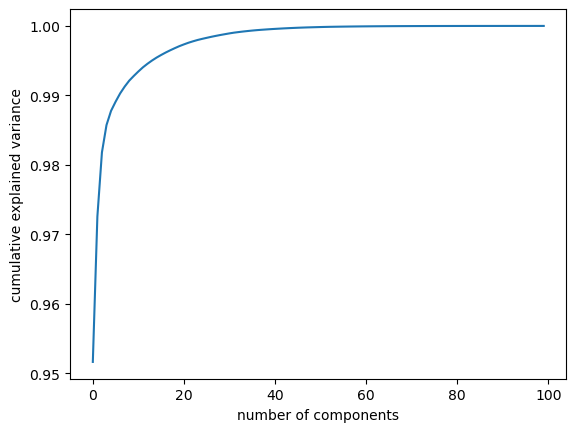
\includegraphics[width=0.7\textwidth]{image/pca.png}}
    \caption{The number of components needed to explain variance
    } \label{fig:no-component-variance}
\end{figure}
From the figure, five number of component should be enough to get most of the dataset variance coverage, 
\subsection{Machine Learning}

\subsubsection{Ridge}
Ridge regression is also a technique used in linear regression, the same as lasso, which is a tool that helps fix tuning models when dealing with closely related data, called a multicollinearity problem\cite{ridge}. It applies L2 regularization to handle this. When data has multicollinearity, standard least-square techniques stay unbiased, but variation grows, which leads to substantial differences between predicted parameter estimation. To deal with this, ridge regression adds some bias to improve the accuracy with which parameters are estimated.
The cost function for ridge regression can be performed like this: 
\begin{quote}
    
    \(J(\theta) = \frac{1}{2m}\sum_{i=1}^{m}((h_{\theta}(x^{(i)} - {y^{(i)})}^{2} + \lambda\sum_{j=1}^{n}\left| \theta_{j} \right|)\)
\end{quote}
    
\begin{itemize}
    \item \(J(\theta)\): cost function
    \item \(m\) number of the training set
    \item \(h_{\theta}(x^{(i)}\)\textbf{)}: predicted output value of
    i\textsuperscript{th} training examples
    \item \(\lambda\): regularization term,
    \item \(n\): number of features,
    \item \(\theta_{j}\): weight of j\textsuperscript{th} feature.

\end{itemize}

Ridge regression works best when having more predicted variables than the observations in the data. This is especially useful in cases where the standard assumptions of linear regression might not be valid. It finds a middle ground between effectively capturing relationships within the data and preventing overfitting issues. 

\subsubsection{Lasso}

Lasso regression is a technique used in regression analysis. Like Ridge Regression, it is a way to shrink and select coefficients in linear regression models, especially with many predictors or multicollinearity. It adds a penalty based on absolute coefficient values ( L1 regularization), which can precisely zero out some coefficients. Effectively performing feature selection. This prevents overfitting, simplifies models, and is great when only a subset of predictors is vital.
\begin{quote}
    
    \(J(\theta) = \frac{1}{2m}\sum_{i=1}^{m}((h_{\theta}(x^{(i)} - {y^{(i)})}^{2} + \lambda_{1}\sum_{j=1}^{n}\theta_{j}^{2} + \lambda_{2}\sum_{j=1}^{n}\theta_{j}^{2})\)
\end{quote}

\begin{itemize}
    \item \(J(\theta)\): cost function
    \item \(m\): number of the training set
    \item \(h_{\theta}(x^{(i)}\)\textbf{)}: predicted output value of
    i\textsuperscript{th} training examples
    \item \(\lambda\): regularization term,
    \item \(n\): number of features,
    \item \(\theta_{j}\): weight of j\textsuperscript{th} feature.

\end{itemize}

What makes Lasso different from Ridge is that while Lasso can lead to zero coefficients, Ridge keeps predictors, although their magnitude is reduced. By ignoring some specific predictors, Lasso is best for its simplicity and clarity, whereas Ridge is well-suited for situations where numerous influential predictors are involved

\subsubsection{ElasticNet}

ElasticNet is a powerful and flexible regularization method which have both characteristics of Lasso and Ridge regression, it merges the capability of dealing with high-dimensionality and the need for robust regularization techniques which means that ElasticNet is the combination of L1 and L2 regularization. By mixing L1 and L2 regularization, it aims to strike a balance between simplicity and retaining relevant predictors. ElasticNet provides two parameters, alpha, and lambda, to balance these two types of regularization. The alpha parameter controls the mix of L1 and L2 regularization, allowing us to emphasize one over the other or find an equilibrium between the two. The lambda parameter controls the overall strength of regularization, controlling how much the coefficients shrink

\begin{quote}
    
    \(J(\theta) = \frac{1}{2m}((h_{\theta}(x^{(i)} - {y^{(i)})}^{2} + \lambda_{1}\theta_{j}^{2} + \lambda_{2}\theta_{j}^{2})\)
\end{quote}


\begin{itemize}
    \item \(J(\theta)\): cost function
    \item \(m\): number of the training set
    \item \(h_{\theta}(x^{(i)}\)\textbf{)}: predicted output value of
    i\textsuperscript{th} training examples
    \item \(y^{(i)}\): real output value of ith training examples,
    \item \(\lambda_{1}\)\textbf{,} \({\ \lambda}_{2}\):: regularization terms,
    \item \(n\): number of features,
    \item \(\theta_{j}\): weight of jth feature.
\end{itemize}

\subsubsection{Decision Tree}
Decision tree is a versatile algorithm used for classification and regression tasks\cite{DecisionTree}. A decision tree is a supervised learning technique mainly applied for classification task machine learning, where the data is represented in a tree-like structure. 

The Decision tree components include Root Node which is the whole dataset where the tree starts. From the root node, the tree will be divided into a subtree known as decision nodes. At the end of a branch will be a leaf node and cannot be split into another branch.

The main advantage of using the decision tree is the algorithm works like a human thinks and makes decisions and is easy to understand due to the tree-like structure. this approach also requires fewer resources to pre-process than other algorithms. However, the number of branches is higher the more complex the data is and contains lots of layers. The bigger the tree, the more the output will be overfitting.

Pruning - With a big tree model, to prevent the data from overfitting, the data will be pruned which is a process to remove branches containing non-important decisions/output of the tree. Cost complexity pruning and reduced error pruning are the most well-known processes. The other known way to reduce the chance of overfitting is using a random forest algorithm.


\begin{figure}[h]
\centering
    \subfigure[]{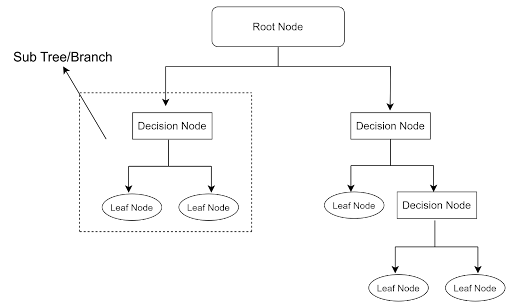
\includegraphics[width=1\textwidth]{image/decision_tree_workflow.png}}
\caption{Decision Tree workflow} \label{fig:decision-tree-workflow}
\end{figure}


The decision tree starts with data preparation, where a dataset with input features and a target variable is collected. It selects initial features as the root node, splits the data based on feature values, and calculates the reduction at each step. When the process chooses the best split, which will become the first split of the tree, it will repeat from the beginning to this step. To make predictions, it goes from branches based on feature values to reach leaf nodes, which contain target value predictions that have averaged. After evaluation with metrics like MSE or R squared, it may apply pruning to refine the tree’s structure. 

\subsubsection{Random Forest}
Random forest is a learning method for regression or classification tasks that construct a decision tree when training \cite{randForest}. 
The random forest algorithms train data while applying the technique of bootstrap aggregating to tree branches to deal with an uncorrelated ensemble of the decision trees. this technique will make sure that each decision tree in the forest is set for a different set of features, by randomly selecting a subset of features from the dataset. 


\begin{figure}[h]
\centering
    \subfigure[]{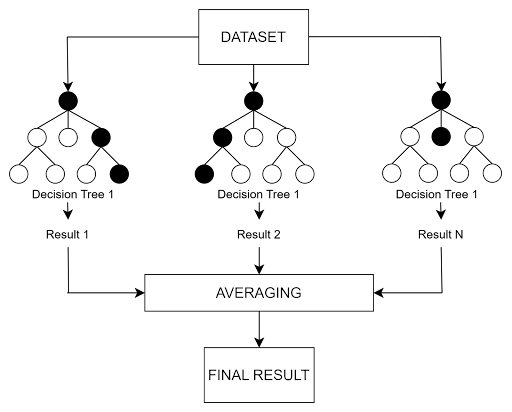
\includegraphics[width=1\textwidth]{image/rand_forrest_workflow.png}}
\caption{Random Forest workflow} \label{fig:rand_forrest_workflow}
\end{figure}

The Random Forest algorithm runs through a bunch of systematic steps to create a predictive model. It starts with data preparation and then uses bootstrapping to create diverse subsets of the data. For each subset, it constructs a decision tree that contains information about the feature randomness, which means that there is only a random subset of features at each node for splitting. Predictions from these trees are combined through averaging for regression and voting for classification to get to the final prediction. The Random Forest model can be working great through parameter adjustments and evaluated using suitable metrics, while also giving a view of feature importance. 

Random Forest brings users several advantages such as their versatility and accuracy when handling diverse data types including binary, numerical, and categorical features, making them robust against outliers and nonlinear features. One of the most useful capabilities is its ability to balance errors in populations and unbalanced datasets, measuring feature importance is straightforward. However, they can be slower due to building many trees, limiting real-time use. The predictions rely on past data and may not work well with different ranges. Also, they are not easy to understand and the decisions cannot be explained easily.

\subsubsection{Support Vector Regression}
Support Vector Regression (SVR) is a specialized type of support vector machine (SVM) used for regression tasks, targeted to predict continuous output values based on given input data. It can be used both for linear and non-linear kernels, with a simple dot product between input vectors for linear kernels while capturing more complex data patterns for non-linear kernels. Choosing between linear and non-linear is based on data characteristics and task complexity. SVR is based on SVM principles, with the same main role being error minimization while finding a hyperplane with a margin that allows for some error. 
This minimization process for the parameter ‘w’ in the equation is akin to maximizing the margin:
\begin{quote}
    \({\min\left| |w| \right|}^{2} + C\sum_{i}^{n}(\xi_{i}^{+} + \ \xi_{i}^{-})\ \ \)
\end{quote}

In order to reduce this error, we utilize the following equation, where the summation component represents an empirical error. 


To minimize the error, we use the following equation:
\begin{quote}
    \(f(x) = \ \sum_{i}^{n}\left( \alpha_{i}^{*} + \ \alpha_{i} \right)K\ \left( x,x_{i} \right) + B\)
\end{quote}
And to calculate the kernel K we can use the following equation: 

\begin{quote}
    \(K\left( x,x_{i} \right) = \ \gamma\left( x*\ x_{i} + 1 \right)^{d}\ \)

\end{quote}

Research with other algorithms shows that SVR acquires better results when working with Linear Regression or ElasticNet. The algorithms also show high accuracy results when working with large datasets with a high number of variables. The SVR has high compatibility when used alongside functions such as geometric, transmission, or data generalization.  Implement standardization is highly recommended when ensuring unbiases evaluations.

\subsubsection{Bayesian Ridge}
Bayesian linear regression predicts the mean of one variable using a weighted sum of others. Its goal is to calculate the posterior probability of regression coefficients and other distribution parameters based on observed predictors.  Bayesian regression suits datasets with sparse or poorly distributed data, as it derives the posterior distribution of model parameters rather than estimating them directly. 
\begin{quote}
    \(p(y\ |\ X,w,a)\  = \ N\ (y\ |\ X_{w}{,a)}_{}\)
\end{quote}
Bayesian Ridge regression, which is the most widely used type of Bayesian regression, models regression problems by incorporating probability estimates. This helps account for uncertainty in predictions, making it useful for situations with limited data or noise. The prior for the coefficients w is given by spherical Gaussian as follows.

\begin{quote}
    \(p(w\ |\ \lambda)\  = \ N\ (w\ |\ 0,\ \lambda^{- 1}I_{p}\))
\end{quote}

\subsubsection{Lasso Lars}
Lasso Lars regression is the mixture of two techniques: Lasso and Lars. 
\paragraph{Lasso} is primarily used for feature selection and addressing multicollinearity in linear regression models. On the other hand, Lars is an algorithm used for efficiently selecting variables in a high-dimensional dataset. Combining these two techniques, Lasso Lars inherits the feature selection capabilities of Lasso and the efficient variable selection process of Lars. This makes it particularly well suited for linear regression tasks involving datasets with many predictor variables or situations where multicollinearity is present. 
It starts with all coefficients at zero and selects predictors based on their correlation with the target variable. As it progresses, it employs Lasso’s feature selection, encouraging some coefficients to become zero, simplifying the model. This approach excels in handling high-dimensional data efficiently while building interpretable and accurate linear regression models.

\paragraph{Lars}

Least Angle Regression (Lars) is used for feature selection and model building, which is specially designed for high dimensional datasets. Its main task is to select and incorporate the most correlated contributions into the model without overfitting. To fit the models, we start by normalizing all values. Then we choose the most highly correlated variable with the residual and adjust the regression line. This process continues until we have used all data or created a satisfactory model. 


\begin{figure}[h]
\centering
    \subfigure[]{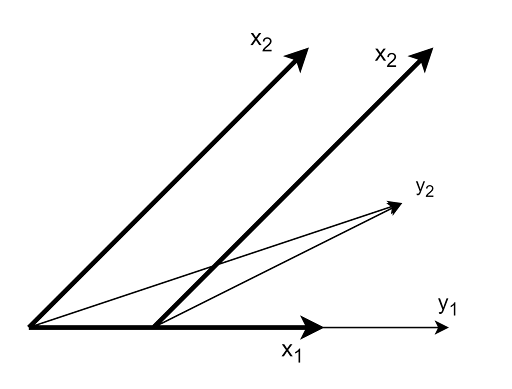
\includegraphics[width=0.8\textwidth]{image/lars.png}}
\caption{Lars Skrinkage} \label{fig:lars}
\end{figure}

\begin{itemize}
    \item y2 is the projection of  y onto L( x1, x2) 
    \item Two covariates x1 and x2 and the space L(x1, x2) that is spanned by them 
    \item Start at \(\mu_{0} = 0\)
\end{itemize}

Firstly, we start with all coefficients as zero and find the predictor variable xj that correlates most with the target variable y. Then we increase the coefficients Bj in the direction of this correlation until another predictor variable xk with equal or higher correlation is found. The coefficients (Bj, Bk) are adjusted so that they have the same angle with xj and xk. This process continues until all predictor variables are included in the model. 

\subsubsection{Boosting}
Boosting is a powerful ensemble meta-algorithm in machine learning that reduces bias and variance in supervised learning. It transforms weak learners into strong ones by combining them iteratively and adjusting their weights based on accuracy. Boosting emerged from the idea of enhancing weak learners to create strong ones. Boosting methods assume training weak classifiers sequentially, making it an essential concept in machine learning and statistics. By each stage of adding, a process called ‘re-weighting’, misclassified data points to gain higher weight, allowing weak learners to focus on them. There are a large number of types of boosting algorithms but in this project, we are supposed to use just the most popular which are AdaBoost, XGBoost, LGBM, CatBoost, and GradientBoost. 


\begin{figure}[h]
\centering
    \subfigure[]{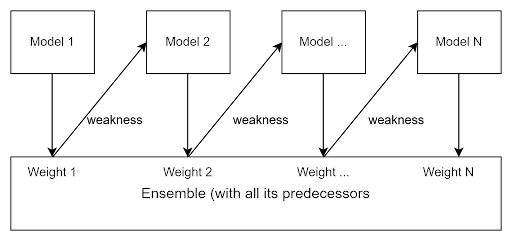
\includegraphics[width=1\textwidth]{image/Boost_workflow.png}}
\caption{Boosting algorithm workflow} \label{fig:Boost_workflow}
\end{figure}


The boosting algorithm contains several advantages, including improved accuracy achieved by combining predictions from weak models, robustness against overfitting by giving more weight to misclassified data points, and effective handling of imbalanced datasets. However, boosting algorithms also have some limitations which can be named as the sensitivity which will make them less suitable when working with real-time applications. Unlike others focused on high-quality predictions, boosting algorithms rely on weak models, each addressing the predecessor’s weaknesses. 


\subsubsection{Gradient Boosting}
Gradient Boosting is a robust boosting algorithm that combines weak learners into strong ones by training each new model to minimize the loss function of the previous model using gradient descent. In each iteration, it calculates the gradient of the loss function regarding the predictions of the current ensemble and trains a new weak model to minimize this gradient. This method often uses decision trees as weak learners to transform the data. The iterative procedure involves computing residuals, which represent the difference between predictions and actual values, and training models to map features to these residuals. These steps are to improve the overall predictive performance of the model. 

We can express how GradientBoosting works through these steps: 

\paragraph*{Step 1:} Assume X and Y are the input and target with N samples. The goal is to find a function f(x) that maps input features X to target variables Y. The loss function quantifies the difference between actual and predicted values
\begin{quote}
    
    \(L(f) = \ \sum_{i=1}^{N}L(y_{i},\ f\left( x_{i} \right))\)
\end{quote}

\paragraph*{Step 2:} Focuses on minimizing L(f) with respect to f
f0x=argmin f  Lf= argmin f  i=1NL(yi, fxi)
In our gradient boosting algorithm with M stages, we improve the model fm by introducing additional estimators denoted as hm, where m ranges from 1 to M
\begin{quote}
    \({\widehat{f}}_{0}(x) = argmin\ f\ \ L(f) = \ argmin\ f\ \ \sum_{i=1}^{N}L(y_{i},\ f\left( x_{i} \right))\)

\end{quote}

\paragraph*{Step 3:} Steepest Descent
\begin{quote}
    \(g_{im} = \  - {\lfloor\frac{\partial L(y_{i},\ f\left( x_{i} \right))}{\partial f(x_{i})}\rfloor}_{f\left( x_{i} \right) = \ f_{m - 1}\ (x_{i})}\)

\end{quote}

With the M stage of Gradient Boosting, the Steepest Descent technique is used to determine the  hm which is an important component. This is the combination of 2 elements: constant termed as step length, and the gradient of the loss function gm. The key point of the step length is to scale the gradient of the loss function L(f). 

\paragraph*{Step 4:} we update the solution iteratively using 
\begin{quote}
    \(f_{m}(x) = \ f_{m - 1}(x) + \left( argmin\ h_{m \in H}\ \ \left\lbrack \sum_{i=1}^{N}L\left( y_{i},\ f_{m - 1}\left( x_{i} \right) + \ h_{m}\left( x_{i} \right) \right) \right\rbrack \right)(x)\)
    
\end{quote}
This process continues for M trees, refining the model at each stage to achieve a more accurate prediction. The solution can also be written as:
\begin{quote}
    \(f_{} = \ f_{m - 1} - \ \rho_{m}g_{m}\)

\end{quote}


\subsubsection{Adaptive Boosting}
AdaBoost, short for Adaptive Boosting is a machine learning algorithm that combines the outputs of weak learners to create a strong classifier. It is known for its adaptability and the ability to handle various base learners including weak ones like decision stumps or even strong learners like deep decision trees, making it versatile. AdaBoost adapts by giving more emphasis to instances that previous learners misclassified, reducing the risk of overfitting. It assigns different weights to errors, influencing the importance of weak learners in the final model. 
This is an example of how AdaBoost works through a pseudocode: 

\begin{quote}
\begin{longtable}[]{@{}
  >{\raggedright\arraybackslash}p{(\columnwidth - 2\tabcolsep) * \real{0.1232}}
  >{\raggedright\arraybackslash}p{(\columnwidth - 2\tabcolsep) * \real{0.8768}}@{}}
\toprule()
\begin{minipage}[b]{\linewidth}\raggedright
\textbf{Input:}
\end{minipage} & \begin{minipage}[b]{\linewidth}\raggedright
Data set
\(D = \left\{ \left( x_{1},\ y_{1} \right),\ \left( x_{2},\ y_{2} \right),\ \ldots\ \left( x_{m},\ y_{m} \right) \right\};\)
\end{minipage} \\
\begin{minipage}[b]{\linewidth}\raggedright
\end{minipage} & \begin{minipage}[b]{\linewidth}\raggedright
Base learning algorithm \(L\);
\end{minipage} \\
\multicolumn{2}{@{}>{\raggedright\arraybackslash}p{(\columnwidth - 2\tabcolsep) * \real{1.0000} + 2\tabcolsep}@{}}{%
\begin{minipage}[b]{\linewidth}\raggedright
\textbf{Output:} \(H(x) = sign(\sum_{t=1}^{T}\alpha_{t}h_{t}(x)\)
\end{minipage}} \\
\begin{minipage}[b]{\linewidth}\raggedright
\end{minipage} & \begin{minipage}[b]{\linewidth}\raggedright
Number of learning round T.
\end{minipage} \\
\begin{minipage}[b]{\linewidth}\raggedright
\textbf{Process:}
\end{minipage} & \begin{minipage}[b]{\linewidth}\raggedright
\end{minipage} \\
\multicolumn{2}{@{}>{\raggedright\arraybackslash}p{(\columnwidth - 2\tabcolsep) * \real{1.0000} + 2\tabcolsep}@{}}{%
\begin{minipage}[b]{\linewidth}\raggedright
\(D_{1}(i) = 1/m\) \% Initialize the weight distribution
\end{minipage}} \\
\multicolumn{2}{@{}>{\raggedright\arraybackslash}p{(\columnwidth - 2\tabcolsep) * \real{1.0000} + 2\tabcolsep}@{}}{%
\begin{minipage}[b]{\linewidth}\raggedright
for \(t = 1,\ \ldots\ ,\ T\);
\end{minipage}} \\
\begin{minipage}[b]{\linewidth}\raggedright
\end{minipage} & \begin{minipage}[b]{\linewidth}\raggedright
\(h_{t} = \ L\left( D,\ D_{t} \right);\ \ \) \% Train a weak learner
\(h_{t}\) from D using distribution \(D_{t}\)
\end{minipage} \\
\begin{minipage}[b]{\linewidth}\raggedright
\end{minipage} & \begin{minipage}[b]{\linewidth}\raggedright
\(\epsilon_{t} = \ \Pr_{i\sim Di}\lbrack h_{t}(x_{i}\  \neq \ y_{i})\rbrack;\)
\% Measure the error of \(h_{t}\)
\end{minipage} \\
\begin{minipage}[b]{\linewidth}\raggedright
\end{minipage} & \begin{minipage}[b]{\linewidth}\raggedright
\(\alpha_{t} = \ \frac{1}{2}\ln\ln\ \left( \frac{1 - \ \epsilon_{t}}{\epsilon_{t}} \right)\ ;\)
\% Determine the weight of the \(h_{t}\)
\end{minipage} \\
\begin{minipage}[b]{\linewidth}\raggedright
\end{minipage} & \begin{minipage}[b]{\linewidth}\raggedright
\(D_{t + 1} = \ \frac{D_{t}(i)}{Z_{t}}\  \times \{\exp\ \left( - \alpha_{t} \right)\ \ if\ h_{t}\left( \ x_{i} \right) = \ y_{i}\ exp\ \left( \alpha_{t} \right)\ \ if\ h_{t}\left( \ x_{i} \right)\  \neq \ y_{i}\ \ \ \ \)

\(= \ \frac{D_{t}(i)exp( - \alpha_{t}y_{i}h_{t}(x_{i})}{Z_{t}}\) \%
update the distribution, where \(Z_{t}\) is

\% a normalization factor which enables \(D_{t + 1}\) be a distribution end.

\end{minipage} \\
\multicolumn{2}{@{}>{\raggedright\arraybackslash}p{(\columnwidth - 2\tabcolsep) * \real{1.0000} + 2\tabcolsep}@{}}{%
\begin{minipage}[b]{\linewidth}\raggedright
\end{minipage}} \\
\midrule()
\endhead
\bottomrule()
\end{longtable}
\end{quote}

AdaBoost offers several advantages, notably its ease of use with minimal parameter tuning, in contrast to more complex algorithms like SVM. However there are some disadvantages, AdaBoost’s progressive learning process demands high-quality data as it’s sensitive to noise and outliers. 



\section{Implementation} \label{implementation}

\subsection{Study Pipeline}

\begin{figure}[h]
\centering
    \subfigure[]{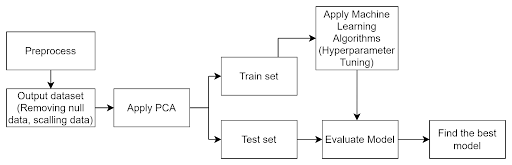
\includegraphics[width=1\textwidth]{image/framework.png}}
\caption{The models workflow} \label{fig:models-workflow}
\end{figure}

First of all, the data need to be prepared before applying with any model. 260 reflectance information files each including 2150 rows of figures. After proccessing the raw data and removing all the null data, the result is an output csv file with 168 row and 2154 collumns. The obtained data may contains features with a variety of dimensions and scales. These differences leads to a biased predictions results in terms of accuracy rates. To avoid this, it is necessary to implement standardization scale to the data before applying to modelin. The next step, the main works of this project, is the analysis and study the relationship of the reflectance data with the plants nutrients. The dataset is splitted into a train set and a test set with a 80-20 portions. To make the model more effective in exploring such a high-dimensional datasets, two methods is proposed. One is using PCA which have been widely used with machine learning algorithms. Others method, limiting which reflectance bandwidth is selected to ran through the models can show the correlation betwween the bandwidth and the plant's nutrient. Since multple models are used in this study, optuna is applied as a tool to automatically find the best hyperparameter for each corresponding models. Finally, the models is continously executed using the dataset that is limited by the red and infra-red bandwidth. From all the collected result, the prediction data and desirable wavelegth, we can conclude which one will be the best model and technique for resolving our challenge.  
 

\subsection{Tools \& Library}
For this project, most of the work is ran using ICTlab servers.
\begin{itemize}
    \item 
    Scikit-learn: Scikitlearn is an open-source machine learning library for Python. It offers several tools for various machine learning tasks including classification, regression, clustering, dimensional reduction, model selection, and data preprocessing. 
    \item 
    Optuna: This is an open-source hyperparameter optimization for machine learning models, which helps in finding the best hyperparameters, making it easier to improve performance and accuracy. Optuna contains various optimization algorithms to search for the optimal hyperparameter in a defined space.
    \item
    Numpy, Matplotlib: used for scientific computing and visualization. Numpy is used for numerical computing and Matplotlib is a tool for creating data visualization.
\end{itemize}

\subsection{Prepare the dataset}
As mentioned above, in this study, two type of dataset need to be put together. First is the main dataset which is the combination of 2 file. The csv file, which contain the measured data of the plant nutrients and its position. The sed file contain most of the information of the vegetation spectral reflectance, however it needs to filter a lot of noise data before merging.
Secondly, another dataset need to generated, the steps remain largely the same, except to analyse which bandwidth is most compatible, the spectral reflectance data need to be limited by the corresponding red and infra red bandwidth. While the highest bandwidth in the dataset is only 2500 nm, the number of time need to ran for each model is over 20000 combination. Most simple model can run through the experiements just fine, However for more advance model, this method could be quite taxing procedure.

\subsection{Hyperparameter Optimization}

Hyperparameter Optimization in Machine learning is the tool to select the best parameters for the learning algorithm. These hyperparameters find the values that can improve the efficiency of model performance. The main idea is to tune parameters to ensure that the model can handle data patterns and minimize a predefined loss function. Cross-validation is commonly used to estimate performance and choose the hyperparameter values that maximize it. There are several ways to optimize hyperparameters such as Grid Search, Random Search, etc. Grid Search is working when specifying a range of parameter values and testing them to see which will work best. This process requires performance metrics like cross-validation to guide the choice. However, when dealing with parameters that can take on real or unbounded values, we may need to set boundaries and discrete values before conducting the grid search. Grid Search is not such a great choice when working with high dimensional parameters space. So to work with more advance model likes AdaBoost, we choose Optuna\cite{optuna}, which is an automatic hyperparameter optimization framework, as a backup plan. Optuna runs based on the define-by-run approach, which will bring flexibility when working with high-dimensional spaces for hyperparameters. 

\subsection{Model Evaluation}

\subsubsection{Mean Squared Error (MSE)}
MSE quantifies the average squared difference between estimated values and actual values. In machine learning, it is one of the popular metrics when evaluating the quality of predictors or estimators. MSE is a non-negative value increasing as errors grow in the model. It considers both variance (how wide estimates vary across data samples) and bias (how far the average between estimates and true value). For an unbiased estimator, MSE equals the variance of the estimator. MSE can be given as the following equation:
\begin{quote}
    
    \(MSE = \frac{1}{n}\ \sum_{i=1}^{n}({\ Y}_{i} - {\widehat{Y}}_{i}\ )^2\)
\end{quote}

\begin{itemize}
    \item \(Y_{i}\): the i\_th observed value,
    \item \({\widehat{Y}}_{i}\): the corresponding predicted value,
    \item \(n\) = the number of observations.
\end{itemize}

\subsubsection{R square}
R squared or R2 (coefficient of determination) is one of the metrics to understand how the output values (variance of a dependent variable) are explained by an independent variable. The value ranges from 0 to 1 and can be negative if the model performs worse than the average fit. An R2 above 0.7 can be signified as a strong correlation, while below 0.4 signified a weaker one. 
\begin{quote}
    \(R^{2} = 1 - \frac{{SS}_{Regression}}{{SS}_{Total}}\)

\end{quote}
\begin{itemize}
    \item \({SS}_{Regression}\) : the sum of squares due to regression,
    \item \({SS}_{Total}\) : the total sum of squares.
\end{itemize}

\subsubsection{Mean Absolute Percentage Error (MAPE)}
Mean Absolute Percentage Error (MAPE) is a metric for evaluating the accuracy of predicting methods, especially when we are working with large and nonzero dataset values. It calculates the percentage error between predicted and actual values. A MAPE below 5\% is a highly accurate prediction, while a MAPE between 10\% and 25\% is acceptable. But when it exceeds 25\%, it means that the results come out have very low accuracy, equivalent to an unacceptable prediction. 

\begin{quote}
    
    \(MAPE = \frac{1}{n} \sum_{t=1}^{n}\left| \frac{A_{t} - F_{t}}{A_{t}} \right|\)
\end{quote}
\begin{itemize}
    \item  \(n\) : sample size,
    \item  \(A_{t}\): the actual data value,
    \item  \(F_{t}\): the forecasted data value.
\end{itemize}

\chapter{Result \& Discussion} \label{chap:result}
\section{Evaluation} \label{section:evaluation}
\subsection{Chlorophyll Model Prediction}


\begin{longtable}[]{@{}
  >{\raggedright\arraybackslash}p{(\columnwidth - 12\tabcolsep) * \real{0.2053}}
  >{\raggedright\arraybackslash}p{(\columnwidth - 12\tabcolsep) * \real{0.1571}}
  >{\raggedright\arraybackslash}p{(\columnwidth - 12\tabcolsep) * \real{0.1104}}
  >{\raggedright\arraybackslash}p{(\columnwidth - 12\tabcolsep) * \real{0.1291}}
  >{\raggedright\arraybackslash}p{(\columnwidth - 12\tabcolsep) * \real{0.1462}}
  >{\raggedright\arraybackslash}p{(\columnwidth - 12\tabcolsep) * \real{0.1104}}
  >{\raggedright\arraybackslash}p{(\columnwidth - 12\tabcolsep) * \real{0.1415}}@{}}
  \toprule()
  \multirow{2}{*}{\begin{minipage}[b]{\linewidth}\raggedright
  Models
  \end{minipage}} &
  \multicolumn{3}{>{\raggedright\arraybackslash}p{(\columnwidth - 12\tabcolsep) * \real{0.3966} + 4\tabcolsep}}{%
  \begin{minipage}[b]{\linewidth}\raggedright
  Without PCA
  \end{minipage}} &
  \multicolumn{3}{>{\raggedright\arraybackslash}p{(\columnwidth - 12\tabcolsep) * \real{0.3981} + 4\tabcolsep}@{}}{%
  \begin{minipage}[b]{\linewidth}\raggedright
  PCA (5 components)
  \end{minipage}} \\
  & \begin{minipage}[b]{\linewidth}\raggedright
  MSE
  \end{minipage} & \begin{minipage}[b]{\linewidth}\raggedright
  R\textsuperscript{2}
  \end{minipage} & \begin{minipage}[b]{\linewidth}\raggedright
  MAPE
  \end{minipage} & \begin{minipage}[b]{\linewidth}\raggedright
  MSE
  \end{minipage} & \begin{minipage}[b]{\linewidth}\raggedright
  R\textsuperscript{2}
  \end{minipage} & \begin{minipage}[b]{\linewidth}\raggedright
  MAPE
  \end{minipage} \\
  \midrule()
  \endhead

\end{longtable}
\begin{longtable}[]{@{}
>{\raggedright\arraybackslash}p{(\columnwidth - 12\tabcolsep) * \real{0.2053}}
>{\raggedright\arraybackslash}p{(\columnwidth - 12\tabcolsep) * \real{0.1571}}
>{\raggedright\arraybackslash}p{(\columnwidth - 12\tabcolsep) * \real{0.1104}}
>{\raggedright\arraybackslash}p{(\columnwidth - 12\tabcolsep) * \real{0.1291}}
>{\raggedright\arraybackslash}p{(\columnwidth - 12\tabcolsep) * \real{0.1462}}
>{\raggedright\arraybackslash}p{(\columnwidth - 12\tabcolsep) * \real{0.1104}}
>{\raggedright\arraybackslash}p{(\columnwidth - 12\tabcolsep) * \real{0.1415}}@{}}
\toprule()
\multirow{2}{*}{\begin{minipage}[b]{\linewidth}\raggedright
Models
\end{minipage}} &
\multicolumn{3}{>{\raggedright\arraybackslash}p{(\columnwidth - 12\tabcolsep) * \real{0.3966} + 4\tabcolsep}}{%
\begin{minipage}[b]{\linewidth}\raggedright
Without PCA
\end{minipage}} &
\multicolumn{3}{>{\raggedright\arraybackslash}p{(\columnwidth - 12\tabcolsep) * \real{0.3981} + 4\tabcolsep}@{}}{%
\begin{minipage}[b]{\linewidth}\raggedright
PCA (5 components)
\end{minipage}} \\
& \begin{minipage}[b]{\linewidth}\raggedright
MSE
\end{minipage} & \begin{minipage}[b]{\linewidth}\raggedright
R\textsuperscript{2}
\end{minipage} & \begin{minipage}[b]{\linewidth}\raggedright
MAPE
\end{minipage} & \begin{minipage}[b]{\linewidth}\raggedright
MSE
\end{minipage} & \begin{minipage}[b]{\linewidth}\raggedright
R\textsuperscript{2}
\end{minipage} & \begin{minipage}[b]{\linewidth}\raggedright
MAPE
\end{minipage} \\
\midrule()
\endhead
\begin{minipage}[b]{\linewidth}\raggedright
Linear Regression
\end{minipage} & \begin{minipage}[b]{\linewidth}\raggedright
10.16
\end{minipage} & \begin{minipage}[b]{\linewidth}\raggedright
-0.00
\end{minipage} & \begin{minipage}[b]{\linewidth}\raggedright
6.38\%
\end{minipage} & \begin{minipage}[b]{\linewidth}\raggedright
9.71
\end{minipage} & \begin{minipage}[b]{\linewidth}\raggedright
0.04
\end{minipage} & \begin{minipage}[b]{\linewidth}\raggedright
6.30\%
\end{minipage} \\
\begin{minipage}[b]{\linewidth}\raggedright
Lasso Regression
\end{minipage} & \begin{minipage}[b]{\linewidth}\raggedright
10.64
\end{minipage} & \begin{minipage}[b]{\linewidth}\raggedright
-0.01
\end{minipage} & \begin{minipage}[b]{\linewidth}\raggedright
6.57\%
\end{minipage} & \begin{minipage}[b]{\linewidth}\raggedright
10.17
\end{minipage} & \begin{minipage}[b]{\linewidth}\raggedright
0.00
\end{minipage} & \begin{minipage}[b]{\linewidth}\raggedright
6.38\%
\end{minipage} \\
\begin{minipage}[b]{\linewidth}\raggedright
Decision Tree
\end{minipage} & \begin{minipage}[b]{\linewidth}\raggedright
11.53
\end{minipage} & \begin{minipage}[b]{\linewidth}\raggedright
-0.09
\end{minipage} & \begin{minipage}[b]{\linewidth}\raggedright
6.69\%
\end{minipage} & \begin{minipage}[b]{\linewidth}\raggedright
10.45
\end{minipage} & \begin{minipage}[b]{\linewidth}\raggedright
-0.03
\end{minipage} & \begin{minipage}[b]{\linewidth}\raggedright
6.57\%
\end{minipage} \\
\begin{minipage}[b]{\linewidth}\raggedright
Random Forest
\end{minipage} & \begin{minipage}[b]{\linewidth}\raggedright
\textbf{9.41}
\end{minipage} & \begin{minipage}[b]{\linewidth}\raggedright
\textbf{0.07}
\end{minipage} & \begin{minipage}[b]{\linewidth}\raggedright
\textbf{6.27\%}
\end{minipage} & \begin{minipage}[b]{\linewidth}\raggedright
9.67
\end{minipage} & \begin{minipage}[b]{\linewidth}\raggedright
0.05
\end{minipage} & \begin{minipage}[b]{\linewidth}\raggedright
6.32\%
\end{minipage} \\
\begin{minipage}[b]{\linewidth}\raggedright
Ridge
\end{minipage} & \begin{minipage}[b]{\linewidth}\raggedright
10.60
\end{minipage} & \begin{minipage}[b]{\linewidth}\raggedright
0.00
\end{minipage} & \begin{minipage}[b]{\linewidth}\raggedright
6.65\%
\end{minipage} & \begin{minipage}[b]{\linewidth}\raggedright
9.95
\end{minipage} & \begin{minipage}[b]{\linewidth}\raggedright
0.02
\end{minipage} & \begin{minipage}[b]{\linewidth}\raggedright
6.48\%
\end{minipage} \\
\begin{minipage}[b]{\linewidth}\raggedright
ElasticNet
\end{minipage} & \begin{minipage}[b]{\linewidth}\raggedright
10.41
\end{minipage} & \begin{minipage}[b]{\linewidth}\raggedright
0.02
\end{minipage} & \begin{minipage}[b]{\linewidth}\raggedright
6.57\%
\end{minipage} & \begin{minipage}[b]{\linewidth}\raggedright
10.17
\end{minipage} & \begin{minipage}[b]{\linewidth}\raggedright
0.00
\end{minipage} & \begin{minipage}[b]{\linewidth}\raggedright
6.38\%
\end{minipage} \\
\begin{minipage}[b]{\linewidth}\raggedright
SVR
\end{minipage} & \begin{minipage}[b]{\linewidth}\raggedright
10.23
\end{minipage} & \begin{minipage}[b]{\linewidth}\raggedright
-0.01
\end{minipage} & \begin{minipage}[b]{\linewidth}\raggedright
6.42\%
\end{minipage} & \begin{minipage}[b]{\linewidth}\raggedright
10.24
\end{minipage} & \begin{minipage}[b]{\linewidth}\raggedright
-0.01
\end{minipage} & \begin{minipage}[b]{\linewidth}\raggedright
6.42\%
\end{minipage} \\
\begin{minipage}[b]{\linewidth}\raggedright
Bayesian Ridge
\end{minipage} & \begin{minipage}[b]{\linewidth}\raggedright
10.17
\end{minipage} & \begin{minipage}[b]{\linewidth}\raggedright
0.00
\end{minipage} & \begin{minipage}[b]{\linewidth}\raggedright
6.38\%
\end{minipage} & \begin{minipage}[b]{\linewidth}\raggedright
10.20
\end{minipage} & \begin{minipage}[b]{\linewidth}\raggedright
-0.01
\end{minipage} & \begin{minipage}[b]{\linewidth}\raggedright
6.44\%
\end{minipage} \\
\begin{minipage}[b]{\linewidth}\raggedright
Gradient Boosting
\end{minipage} & \begin{minipage}[b]{\linewidth}\raggedright
9.97
\end{minipage} & \begin{minipage}[b]{\linewidth}\raggedright
0.02
\end{minipage} & \begin{minipage}[b]{\linewidth}\raggedright
6.42\%
\end{minipage} & \begin{minipage}[b]{\linewidth}\raggedright
10.84
\end{minipage} & \begin{minipage}[b]{\linewidth}\raggedright
-0.07
\end{minipage} & \begin{minipage}[b]{\linewidth}\raggedright
6.74\%
\end{minipage} \\
\begin{minipage}[b]{\linewidth}\raggedright
Lasso Lars
\end{minipage} & \begin{minipage}[b]{\linewidth}\raggedright
10.17
\end{minipage} & \begin{minipage}[b]{\linewidth}\raggedright
0.00
\end{minipage} & \begin{minipage}[b]{\linewidth}\raggedright
6.38\%
\end{minipage} & \begin{minipage}[b]{\linewidth}\raggedright
10.18
\end{minipage} & \begin{minipage}[b]{\linewidth}\raggedright
0.00
\end{minipage} & \begin{minipage}[b]{\linewidth}\raggedright
6.41\%
\end{minipage} \\
\begin{minipage}[b]{\linewidth}\raggedright
Lars
\end{minipage} & \begin{minipage}[b]{\linewidth}\raggedright
10.64
\end{minipage} & \begin{minipage}[b]{\linewidth}\raggedright
-0.01
\end{minipage} & \begin{minipage}[b]{\linewidth}\raggedright
6.57\%
\end{minipage} & \begin{minipage}[b]{\linewidth}\raggedright
9.95
\end{minipage} & \begin{minipage}[b]{\linewidth}\raggedright
0.02
\end{minipage} & \begin{minipage}[b]{\linewidth}\raggedright
6.48\%
\end{minipage} \\
\begin{minipage}[b]{\linewidth}\raggedright
AdaBoost
\end{minipage} & \begin{minipage}[b]{\linewidth}\raggedright
11.10
\end{minipage} & \begin{minipage}[b]{\linewidth}\raggedright
-0.05
\end{minipage} & \begin{minipage}[b]{\linewidth}\raggedright
6.52\%
\end{minipage} & \begin{minipage}[b]{\linewidth}\raggedright
\textbf{9.55}
\end{minipage} & \begin{minipage}[b]{\linewidth}\raggedright
\textbf{0.06}
\end{minipage} & \begin{minipage}[b]{\linewidth}\raggedright
\textbf{6.28\%}
\end{minipage} \\
\midrule()
\endhead
\bottomrule()
\caption{Comparison of Learning Models Performance in Chlorophyll Prediction} \label{fig:result-Chlorophyll-pca}

\end{longtable}
\newpage
The Chlorophyll performance with the dataset basically is strong with a quite low result in MAPE of less than 7\% for most of the models, some have higher MAPE result, especially after applying 5 PCA component. Among the models, the Random Forest model without applying PCA seems to be the top performer (with a score of 9.41 of MSE, the highest \(R^2\)  score, and a MAPE of 6.27\% which is also the best one). Though after using PCA with 5 components, while it still have decent score, Random Forest (with 9.41 MSE) is outperformed by AdaBoost which have 6.28\% MAPE score. With this result, we can conclude that the boosting algorithms are the most well-suited to the dataset when . For the machine learning algorithm, there is nothing better than the result of Random Forest without PCA when it has 6.27\% in MAPE, 9.41 in MSE and the \(R^2\) score is 0.07 which is also a good score. When taking a look at the higher number of PCA components, we can see that the result seems to be better in some models, especially with AdaBoosting when the MSE score increases impressively (from 11.10 to 9.55 in MSE score ) through each higher stage of PCA. The results in MAPE and MSE are more stable than with the lower number of components which is around 10 in MSE and around 6.5 in MSE. If choosing one best model for 5 PCA components, AdaBoost, and Linear Regression, among them, Linear Regression seems to have the overall results pretty well. The worst performance is Decision Tree without applying PCA's results (with -0.82 in  \(R^2\) score, the highest MSE 11.53, and the highest MAPE 6.69\%.). After applying PCA the results are much better but still not very desirable MSE: 10.45, \(R^2\): -0.03, MAPE: 6.57\%. The other noticable bad performance is the Gradient Boosting after applying 5 component of PCA MSE: 10.84, \(R^2\): -0.07, MAPE: 6.74\%.

Overall Chlorophyll seems to have the best performance for machine learning models because of having the best result when compared with P and K concentrations.

\begin{longtable}[]{@{}
  >{\raggedright\arraybackslash}p{(\columnwidth - 10\tabcolsep) * \real{0.1883}}
  >{\raggedright\arraybackslash}p{(\columnwidth - 10\tabcolsep) * \real{0.1623}}
  >{\raggedright\arraybackslash}p{(\columnwidth - 10\tabcolsep) * \real{0.1623}}
  >{\raggedright\arraybackslash}p{(\columnwidth - 10\tabcolsep) * \real{0.1623}}
  >{\raggedright\arraybackslash}p{(\columnwidth - 10\tabcolsep) * \real{0.1623}}
  >{\raggedright\arraybackslash}p{(\columnwidth - 10\tabcolsep) * \real{0.1623}}@{}}
\toprule()
\begin{minipage}[b]{\linewidth}\raggedright
Methods
\end{minipage} & \begin{minipage}[b]{\linewidth}\raggedright
Red bw
\end{minipage} & \begin{minipage}[b]{\linewidth}\raggedright
IR bw
\end{minipage} & \begin{minipage}[b]{\linewidth}\raggedright
R square
\end{minipage} & \begin{minipage}[b]{\linewidth}\raggedright
MSE
\end{minipage} & \begin{minipage}[b]{\linewidth}\raggedright
MAPE
\end{minipage} \\
\midrule()
\endhead
\begin{minipage}[b]{\linewidth}\raggedright
Gradient Boost
\end{minipage} & \begin{minipage}[b]{\linewidth}\raggedright
735
\end{minipage} & \begin{minipage}[b]{\linewidth}\raggedright
1084
\end{minipage} & \begin{minipage}[b]{\linewidth}\raggedright
0.03
\end{minipage} & \begin{minipage}[b]{\linewidth}\raggedright
8.299285863
\end{minipage} & \begin{minipage}[b]{\linewidth}\raggedright
5.28\%
\end{minipage} \\
\begin{minipage}[b]{\linewidth}\raggedright
Gradient Boost
\end{minipage} & \begin{minipage}[b]{\linewidth}\raggedright
738
\end{minipage} & \begin{minipage}[b]{\linewidth}\raggedright
1093
\end{minipage} & \begin{minipage}[b]{\linewidth}\raggedright
0.03
\end{minipage} & \begin{minipage}[b]{\linewidth}\raggedright
8.28778986
\end{minipage} & \begin{minipage}[b]{\linewidth}\raggedright
5.30\%
\end{minipage} \\
\begin{minipage}[b]{\linewidth}\raggedright
Gradient Boost
\end{minipage} & \begin{minipage}[b]{\linewidth}\raggedright
730
\end{minipage} & \begin{minipage}[b]{\linewidth}\raggedright
1084
\end{minipage} & \begin{minipage}[b]{\linewidth}\raggedright
0.03
\end{minipage} & \begin{minipage}[b]{\linewidth}\raggedright
8.275941423
\end{minipage} & \begin{minipage}[b]{\linewidth}\raggedright
5.30\%
\end{minipage} \\
\begin{minipage}[b]{\linewidth}\raggedright
Gradient Boost
\end{minipage} & \begin{minipage}[b]{\linewidth}\raggedright
730
\end{minipage} & \begin{minipage}[b]{\linewidth}\raggedright
1094
\end{minipage} & \begin{minipage}[b]{\linewidth}\raggedright
0.03
\end{minipage} & \begin{minipage}[b]{\linewidth}\raggedright
8.286555199
\end{minipage} & \begin{minipage}[b]{\linewidth}\raggedright
5.30\%
\end{minipage} \\
\begin{minipage}[b]{\linewidth}\raggedright
Gradient Boost
\end{minipage} & \begin{minipage}[b]{\linewidth}\raggedright
737
\end{minipage} & \begin{minipage}[b]{\linewidth}\raggedright
1084
\end{minipage} & \begin{minipage}[b]{\linewidth}\raggedright
0.03
\end{minipage} & \begin{minipage}[b]{\linewidth}\raggedright
8.311230227
\end{minipage} & \begin{minipage}[b]{\linewidth}\raggedright
5.30\%
\end{minipage} \\
\begin{minipage}[b]{\linewidth}\raggedright
Random Forrest
\end{minipage} & \begin{minipage}[b]{\linewidth}\raggedright
680
\end{minipage} & \begin{minipage}[b]{\linewidth}\raggedright
1665
\end{minipage} & \begin{minipage}[b]{\linewidth}\raggedright
-0.01
\end{minipage} & \begin{minipage}[b]{\linewidth}\raggedright
8.67683125
\end{minipage} & \begin{minipage}[b]{\linewidth}\raggedright
5.53\%
\end{minipage} \\
\begin{minipage}[b]{\linewidth}\raggedright
Random Forrest
\end{minipage} & \begin{minipage}[b]{\linewidth}\raggedright
650
\end{minipage} & \begin{minipage}[b]{\linewidth}\raggedright
1067
\end{minipage} & \begin{minipage}[b]{\linewidth}\raggedright
0.01
\end{minipage} & \begin{minipage}[b]{\linewidth}\raggedright
8.493064482
\end{minipage} & \begin{minipage}[b]{\linewidth}\raggedright
5.54\%
\end{minipage} \\
\begin{minipage}[b]{\linewidth}\raggedright
Random Forrest
\end{minipage} & \begin{minipage}[b]{\linewidth}\raggedright
642
\end{minipage} & \begin{minipage}[b]{\linewidth}\raggedright
764
\end{minipage} & \begin{minipage}[b]{\linewidth}\raggedright
0
\end{minipage} & \begin{minipage}[b]{\linewidth}\raggedright
8.588484947
\end{minipage} & \begin{minipage}[b]{\linewidth}\raggedright
5.54\%
\end{minipage} \\
\begin{minipage}[b]{\linewidth}\raggedright
Random Forrest
\end{minipage} & \begin{minipage}[b]{\linewidth}\raggedright
677
\end{minipage} & \begin{minipage}[b]{\linewidth}\raggedright
937
\end{minipage} & \begin{minipage}[b]{\linewidth}\raggedright
0
\end{minipage} & \begin{minipage}[b]{\linewidth}\raggedright
8.516774513
\end{minipage} & \begin{minipage}[b]{\linewidth}\raggedright
5.55\%
\end{minipage} \\
\begin{minipage}[b]{\linewidth}\raggedright
Random Forrest
\end{minipage} & \begin{minipage}[b]{\linewidth}\raggedright
637
\end{minipage} & \begin{minipage}[b]{\linewidth}\raggedright
1300
\end{minipage} & \begin{minipage}[b]{\linewidth}\raggedright
0
\end{minipage} & \begin{minipage}[b]{\linewidth}\raggedright
8.527544172
\end{minipage} & \begin{minipage}[b]{\linewidth}\raggedright
5.55\%
\end{minipage} \\
\begin{minipage}[b]{\linewidth}\raggedright
SVR
\end{minipage} & \begin{minipage}[b]{\linewidth}\raggedright
625
\end{minipage} & \begin{minipage}[b]{\linewidth}\raggedright
750
\end{minipage} & \begin{minipage}[b]{\linewidth}\raggedright
-0.19
\end{minipage} & \begin{minipage}[b]{\linewidth}\raggedright
10.15272789
\end{minipage} & \begin{minipage}[b]{\linewidth}\raggedright
5.77\%
\end{minipage} \\
\begin{minipage}[b]{\linewidth}\raggedright
SVR
\end{minipage} & \begin{minipage}[b]{\linewidth}\raggedright
625
\end{minipage} & \begin{minipage}[b]{\linewidth}\raggedright
750
\end{minipage} & \begin{minipage}[b]{\linewidth}\raggedright
-0.19
\end{minipage} & \begin{minipage}[b]{\linewidth}\raggedright
10.15272789
\end{minipage} & \begin{minipage}[b]{\linewidth}\raggedright
5.77\%
\end{minipage} \\
\begin{minipage}[b]{\linewidth}\raggedright
SVR
\end{minipage} & \begin{minipage}[b]{\linewidth}\raggedright
625
\end{minipage} & \begin{minipage}[b]{\linewidth}\raggedright
766
\end{minipage} & \begin{minipage}[b]{\linewidth}\raggedright
-0.16
\end{minipage} & \begin{minipage}[b]{\linewidth}\raggedright
9.890171071
\end{minipage} & \begin{minipage}[b]{\linewidth}\raggedright
5.78\%
\end{minipage} \\
\begin{minipage}[b]{\linewidth}\raggedright
SVR
\end{minipage} & \begin{minipage}[b]{\linewidth}\raggedright
625
\end{minipage} & \begin{minipage}[b]{\linewidth}\raggedright
765
\end{minipage} & \begin{minipage}[b]{\linewidth}\raggedright
-0.16
\end{minipage} & \begin{minipage}[b]{\linewidth}\raggedright
9.910342117
\end{minipage} & \begin{minipage}[b]{\linewidth}\raggedright
5.78\%
\end{minipage} \\
\begin{minipage}[b]{\linewidth}\raggedright
SVR
\end{minipage} & \begin{minipage}[b]{\linewidth}\raggedright
625
\end{minipage} & \begin{minipage}[b]{\linewidth}\raggedright
764
\end{minipage} & \begin{minipage}[b]{\linewidth}\raggedright
-0.16
\end{minipage} & \begin{minipage}[b]{\linewidth}\raggedright
9.928388891
\end{minipage} & \begin{minipage}[b]{\linewidth}\raggedright
5.78\%
\end{minipage} \\
\begin{minipage}[b]{\linewidth}\raggedright
Linear Regression
\end{minipage} & \begin{minipage}[b]{\linewidth}\raggedright
740
\end{minipage} & \begin{minipage}[b]{\linewidth}\raggedright
758
\end{minipage} & \begin{minipage}[b]{\linewidth}\raggedright
-0.22
\end{minipage} & \begin{minipage}[b]{\linewidth}\raggedright
10.46803389
\end{minipage} & \begin{minipage}[b]{\linewidth}\raggedright
5.83\%
\end{minipage} \\
\begin{minipage}[b]{\linewidth}\raggedright
Linear Regression
\end{minipage} & \begin{minipage}[b]{\linewidth}\raggedright
740
\end{minipage} & \begin{minipage}[b]{\linewidth}\raggedright
757
\end{minipage} & \begin{minipage}[b]{\linewidth}\raggedright
-0.22
\end{minipage} & \begin{minipage}[b]{\linewidth}\raggedright
10.47387994
\end{minipage} & \begin{minipage}[b]{\linewidth}\raggedright
5.86\%
\end{minipage} \\
\begin{minipage}[b]{\linewidth}\raggedright
Ridge
\end{minipage} & \begin{minipage}[b]{\linewidth}\raggedright
740
\end{minipage} & \begin{minipage}[b]{\linewidth}\raggedright
756
\end{minipage} & \begin{minipage}[b]{\linewidth}\raggedright
-0.17
\end{minipage} & \begin{minipage}[b]{\linewidth}\raggedright
10.02904318
\end{minipage} & \begin{minipage}[b]{\linewidth}\raggedright
5.91\%
\end{minipage} \\
\begin{minipage}[b]{\linewidth}\raggedright
Ridge
\end{minipage} & \begin{minipage}[b]{\linewidth}\raggedright
740
\end{minipage} & \begin{minipage}[b]{\linewidth}\raggedright
750
\end{minipage} & \begin{minipage}[b]{\linewidth}\raggedright
-0.17
\end{minipage} & \begin{minipage}[b]{\linewidth}\raggedright
10.02936277
\end{minipage} & \begin{minipage}[b]{\linewidth}\raggedright
5.91\%
\end{minipage} \\
\begin{minipage}[b]{\linewidth}\raggedright
Ridge
\end{minipage} & \begin{minipage}[b]{\linewidth}\raggedright
740
\end{minipage} & \begin{minipage}[b]{\linewidth}\raggedright
751
\end{minipage} & \begin{minipage}[b]{\linewidth}\raggedright
-0.17
\end{minipage} & \begin{minipage}[b]{\linewidth}\raggedright
10.03365566
\end{minipage} & \begin{minipage}[b]{\linewidth}\raggedright
5.91\%
\end{minipage} \\
\begin{minipage}[b]{\linewidth}\raggedright
Ridge
\end{minipage} & \begin{minipage}[b]{\linewidth}\raggedright
740
\end{minipage} & \begin{minipage}[b]{\linewidth}\raggedright
752
\end{minipage} & \begin{minipage}[b]{\linewidth}\raggedright
-0.17
\end{minipage} & \begin{minipage}[b]{\linewidth}\raggedright
10.03727319
\end{minipage} & \begin{minipage}[b]{\linewidth}\raggedright
5.91\%
\end{minipage} \\
\begin{minipage}[b]{\linewidth}\raggedright
Ridge
\end{minipage} & \begin{minipage}[b]{\linewidth}\raggedright
740
\end{minipage} & \begin{minipage}[b]{\linewidth}\raggedright
755
\end{minipage} & \begin{minipage}[b]{\linewidth}\raggedright
-0.17
\end{minipage} & \begin{minipage}[b]{\linewidth}\raggedright
10.03919053
\end{minipage} & \begin{minipage}[b]{\linewidth}\raggedright
5.91\%
\end{minipage} \\
\begin{minipage}[b]{\linewidth}\raggedright
Linear Regression
\end{minipage} & \begin{minipage}[b]{\linewidth}\raggedright
740
\end{minipage} & \begin{minipage}[b]{\linewidth}\raggedright
759
\end{minipage} & \begin{minipage}[b]{\linewidth}\raggedright
-0.26
\end{minipage} & \begin{minipage}[b]{\linewidth}\raggedright
10.7475421
\end{minipage} & \begin{minipage}[b]{\linewidth}\raggedright
5.92\%
\end{minipage} \\
\begin{minipage}[b]{\linewidth}\raggedright
Linear Regression
\end{minipage} & \begin{minipage}[b]{\linewidth}\raggedright
740
\end{minipage} & \begin{minipage}[b]{\linewidth}\raggedright
754
\end{minipage} & \begin{minipage}[b]{\linewidth}\raggedright
-0.27
\end{minipage} & \begin{minipage}[b]{\linewidth}\raggedright
10.83335362
\end{minipage} & \begin{minipage}[b]{\linewidth}\raggedright
5.94\%
\end{minipage} \\
\begin{minipage}[b]{\linewidth}\raggedright
Linear Regression
\end{minipage} & \begin{minipage}[b]{\linewidth}\raggedright
740
\end{minipage} & \begin{minipage}[b]{\linewidth}\raggedright
756
\end{minipage} & \begin{minipage}[b]{\linewidth}\raggedright
-0.27
\end{minipage} & \begin{minipage}[b]{\linewidth}\raggedright
10.8463624
\end{minipage} & \begin{minipage}[b]{\linewidth}\raggedright
5.98\%
\end{minipage} \\
\begin{minipage}[b]{\linewidth}\raggedright
Elasticnet
\end{minipage} & \begin{minipage}[b]{\linewidth}\raggedright
660
\end{minipage} & \begin{minipage}[b]{\linewidth}\raggedright
1426
\end{minipage} & \begin{minipage}[b]{\linewidth}\raggedright
-0.03
\end{minipage} & \begin{minipage}[b]{\linewidth}\raggedright
10.31318804
\end{minipage} & \begin{minipage}[b]{\linewidth}\raggedright
6.33\%
\end{minipage} \\
\begin{minipage}[b]{\linewidth}\raggedright
Elasticnet
\end{minipage} & \begin{minipage}[b]{\linewidth}\raggedright
661
\end{minipage} & \begin{minipage}[b]{\linewidth}\raggedright
1426
\end{minipage} & \begin{minipage}[b]{\linewidth}\raggedright
-0.03
\end{minipage} & \begin{minipage}[b]{\linewidth}\raggedright
10.31316867
\end{minipage} & \begin{minipage}[b]{\linewidth}\raggedright
6.33\%
\end{minipage} \\
\begin{minipage}[b]{\linewidth}\raggedright
Elasticnet
\end{minipage} & \begin{minipage}[b]{\linewidth}\raggedright
659
\end{minipage} & \begin{minipage}[b]{\linewidth}\raggedright
1426
\end{minipage} & \begin{minipage}[b]{\linewidth}\raggedright
-0.03
\end{minipage} & \begin{minipage}[b]{\linewidth}\raggedright
10.31320883
\end{minipage} & \begin{minipage}[b]{\linewidth}\raggedright
6.33\%
\end{minipage} \\
\begin{minipage}[b]{\linewidth}\raggedright
Elasticnet
\end{minipage} & \begin{minipage}[b]{\linewidth}\raggedright
658
\end{minipage} & \begin{minipage}[b]{\linewidth}\raggedright
1426
\end{minipage} & \begin{minipage}[b]{\linewidth}\raggedright
-0.03
\end{minipage} & \begin{minipage}[b]{\linewidth}\raggedright
10.31320323
\end{minipage} & \begin{minipage}[b]{\linewidth}\raggedright
6.33\%
\end{minipage} \\
\begin{minipage}[b]{\linewidth}\raggedright
Elasticnet
\end{minipage} & \begin{minipage}[b]{\linewidth}\raggedright
657
\end{minipage} & \begin{minipage}[b]{\linewidth}\raggedright
1426
\end{minipage} & \begin{minipage}[b]{\linewidth}\raggedright
-0.03
\end{minipage} & \begin{minipage}[b]{\linewidth}\raggedright
10.31320132
\end{minipage} & \begin{minipage}[b]{\linewidth}\raggedright
6.33\%
\end{minipage} \\
\midrule()
\bottomrule()
\caption{Best NDVI result from Learning Models in Chlorophyll Prediction} \label{fig:result-Chlorophyll-ndvi}


\end{longtable}




While applying PCA have quite a good influence on the result, manually limitting the spectral bandwidth showed even greatter improvement to the result. After running through multiple model with different combination of red and infrared bandwidth, the best scores is consistantly achieved using GradientBoosting model in 735-1084nm bandwidth. While the R square result still not as good as using PCA, the model's  others score received quite substantial improvement  with MSE: 8.3 and MAPE: 5.28\%. Overall, eventhough the improvements are vary, all other regression has shown possitive developments, each in a different bandwidth range: Random Forest at 680-1665nm, SVR at 625-750, Linear Regression: 740-758nm, Ridge: 740-756nm and ElasticNet: 660-1426nm.

\newpage
\subsection{Phosphorus Model Prediction}

\begin{longtable}[]{@{}
>{\raggedright\arraybackslash}p{(\columnwidth - 12\tabcolsep) * \real{0.2053}}
>{\raggedright\arraybackslash}p{(\columnwidth - 12\tabcolsep) * \real{0.1571}}
>{\raggedright\arraybackslash}p{(\columnwidth - 12\tabcolsep) * \real{0.1104}}
>{\raggedright\arraybackslash}p{(\columnwidth - 12\tabcolsep) * \real{0.1291}}
>{\raggedright\arraybackslash}p{(\columnwidth - 12\tabcolsep) * \real{0.1462}}
>{\raggedright\arraybackslash}p{(\columnwidth - 12\tabcolsep) * \real{0.1104}}
>{\raggedright\arraybackslash}p{(\columnwidth - 12\tabcolsep) * \real{0.1415}}@{}}
\toprule()
\multirow{2}{*}{\begin{minipage}[b]{\linewidth}\raggedright
Models
\end{minipage}} &
\multicolumn{3}{>{\raggedright\arraybackslash}p{(\columnwidth - 12\tabcolsep) * \real{0.3966} + 4\tabcolsep}}{%
\begin{minipage}[b]{\linewidth}\raggedright
Without PCA
\end{minipage}} &
\multicolumn{3}{>{\raggedright\arraybackslash}p{(\columnwidth - 12\tabcolsep) * \real{0.3981} + 4\tabcolsep}@{}}{%
\begin{minipage}[b]{\linewidth}\raggedright
PCA (5 components)
\end{minipage}} \\
& \begin{minipage}[b]{\linewidth}\raggedright
MSE
\end{minipage} & \begin{minipage}[b]{\linewidth}\raggedright
R\textsuperscript{2}
\end{minipage} & \begin{minipage}[b]{\linewidth}\raggedright
MAPE
\end{minipage} & \begin{minipage}[b]{\linewidth}\raggedright
MSE
\end{minipage} & \begin{minipage}[b]{\linewidth}\raggedright
R\textsuperscript{2}
\end{minipage} & \begin{minipage}[b]{\linewidth}\raggedright
MAPE
\end{minipage} \\
\midrule()
\endhead
\begin{minipage}[b]{\linewidth}\raggedright
Linear Regression
\end{minipage} & \begin{minipage}[b]{\linewidth}\raggedright
600400.27
\end{minipage} & \begin{minipage}[b]{\linewidth}\raggedright
0.01
\end{minipage} & \begin{minipage}[b]{\linewidth}\raggedright
17.85\%
\end{minipage} & \begin{minipage}[b]{\linewidth}\raggedright
602786.91
\end{minipage} & \begin{minipage}[b]{\linewidth}\raggedright
0.01
\end{minipage} & \begin{minipage}[b]{\linewidth}\raggedright
17.58\%
\end{minipage} \\
\begin{minipage}[b]{\linewidth}\raggedright
Lasso Regression
\end{minipage} & \begin{minipage}[b]{\linewidth}\raggedright
809576.62
\end{minipage} & \begin{minipage}[b]{\linewidth}\raggedright
0.00
\end{minipage} & \begin{minipage}[b]{\linewidth}\raggedright
21.79\%
\end{minipage} & \begin{minipage}[b]{\linewidth}\raggedright
606748.22
\end{minipage} & \begin{minipage}[b]{\linewidth}\raggedright
0.00
\end{minipage} & \begin{minipage}[b]{\linewidth}\raggedright
17.61\%
\end{minipage} \\
\begin{minipage}[b]{\linewidth}\raggedright
Decision Tree
\end{minipage} & \begin{minipage}[b]{\linewidth}\raggedright
798576.62
\end{minipage} & \begin{minipage}[b]{\linewidth}\raggedright
0.01
\end{minipage} & \begin{minipage}[b]{\linewidth}\raggedright
21.57\%
\end{minipage} & \begin{minipage}[b]{\linewidth}\raggedright
642453.51
\end{minipage} & \begin{minipage}[b]{\linewidth}\raggedright
-0.06
\end{minipage} & \begin{minipage}[b]{\linewidth}\raggedright
18.60\%
\end{minipage} \\
\begin{minipage}[b]{\linewidth}\raggedright
Random Forest
\end{minipage} & \begin{minipage}[b]{\linewidth}\raggedright
673434.06
\end{minipage} & \begin{minipage}[b]{\linewidth}\raggedright
-0.11
\end{minipage} & \begin{minipage}[b]{\linewidth}\raggedright
18,71\%
\end{minipage} & \begin{minipage}[b]{\linewidth}\raggedright
685801.38
\end{minipage} & \begin{minipage}[b]{\linewidth}\raggedright
-0.13
\end{minipage} & \begin{minipage}[b]{\linewidth}\raggedright
18.53\%
\end{minipage} \\
\begin{minipage}[b]{\linewidth}\raggedright
Ridge
\end{minipage} & \begin{minipage}[b]{\linewidth}\raggedright
779860.59
\end{minipage} & \begin{minipage}[b]{\linewidth}\raggedright
0.03
\end{minipage} & \begin{minipage}[b]{\linewidth}\raggedright
21.29\%
\end{minipage} & \begin{minipage}[b]{\linewidth}\raggedright
622814.65
\end{minipage} & \begin{minipage}[b]{\linewidth}\raggedright
-0.03
\end{minipage} & \begin{minipage}[b]{\linewidth}\raggedright
17.81\%
\end{minipage} \\
\begin{minipage}[b]{\linewidth}\raggedright
ElasticNet
\end{minipage} & \begin{minipage}[b]{\linewidth}\raggedright
805652.41
\end{minipage} & \begin{minipage}[b]{\linewidth}\raggedright
0.00
\end{minipage} & \begin{minipage}[b]{\linewidth}\raggedright
21.52\%
\end{minipage} & \begin{minipage}[b]{\linewidth}\raggedright
614590.82
\end{minipage} & \begin{minipage}[b]{\linewidth}\raggedright
-0.01
\end{minipage} & \begin{minipage}[b]{\linewidth}\raggedright
17.72\%
\end{minipage} \\
\begin{minipage}[b]{\linewidth}\raggedright
SVR
\end{minipage} & \begin{minipage}[b]{\linewidth}\raggedright
661599.95
\end{minipage} & \begin{minipage}[b]{\linewidth}\raggedright
-0.09
\end{minipage} & \begin{minipage}[b]{\linewidth}\raggedright
18.24\%
\end{minipage} & \begin{minipage}[b]{\linewidth}\raggedright
636115.22
\end{minipage} & \begin{minipage}[b]{\linewidth}\raggedright
-0.05
\end{minipage} & \begin{minipage}[b]{\linewidth}\raggedright
17.94\%
\end{minipage} \\
\begin{minipage}[b]{\linewidth}\raggedright
Bayesian Ridge
\end{minipage} & \begin{minipage}[b]{\linewidth}\raggedright
\textbf{591150.94}
\end{minipage} & \begin{minipage}[b]{\linewidth}\raggedright
\textbf{0.03}
\end{minipage} & \begin{minipage}[b]{\linewidth}\raggedright
\textbf{17.56\%}
\end{minipage} & \begin{minipage}[b]{\linewidth}\raggedright
\textbf{591923.27}
\end{minipage} & \begin{minipage}[b]{\linewidth}\raggedright
\textbf{0.03}
\end{minipage} & \begin{minipage}[b]{\linewidth}\raggedright
\textbf{17.57\%}
\end{minipage} \\
\begin{minipage}[b]{\linewidth}\raggedright
Gradient Boosting
\end{minipage} & \begin{minipage}[b]{\linewidth}\raggedright
615169.00
\end{minipage} & \begin{minipage}[b]{\linewidth}\raggedright
0.02
\end{minipage} & \begin{minipage}[b]{\linewidth}\raggedright
17.94\%
\end{minipage} & \begin{minipage}[b]{\linewidth}\raggedright
644217.55
\end{minipage} & \begin{minipage}[b]{\linewidth}\raggedright
-0.06
\end{minipage} & \begin{minipage}[b]{\linewidth}\raggedright
18.41\%
\end{minipage} \\
\begin{minipage}[b]{\linewidth}\raggedright
Lasso Lars
\end{minipage} & \begin{minipage}[b]{\linewidth}\raggedright
627916.94
\end{minipage} & \begin{minipage}[b]{\linewidth}\raggedright
-0.33
\end{minipage} & \begin{minipage}[b]{\linewidth}\raggedright
18.21\%
\end{minipage} & \begin{minipage}[b]{\linewidth}\raggedright
622582.18
\end{minipage} & \begin{minipage}[b]{\linewidth}\raggedright
-0.02
\end{minipage} & \begin{minipage}[b]{\linewidth}\raggedright
17.81\%
\end{minipage} \\
\begin{minipage}[b]{\linewidth}\raggedright
Lars
\end{minipage} & \begin{minipage}[b]{\linewidth}\raggedright
831396.92
\end{minipage} & \begin{minipage}[b]{\linewidth}\raggedright
-0.03
\end{minipage} & \begin{minipage}[b]{\linewidth}\raggedright
22.05\%
\end{minipage} & \begin{minipage}[b]{\linewidth}\raggedright
622791.61
\end{minipage} & \begin{minipage}[b]{\linewidth}\raggedright
-0.03
\end{minipage} & \begin{minipage}[b]{\linewidth}\raggedright
17.81\%
\end{minipage} \\
\begin{minipage}[b]{\linewidth}\raggedright
AdaBoost
\end{minipage} & \begin{minipage}[b]{\linewidth}\raggedright
793464.37
\end{minipage} & \begin{minipage}[b]{\linewidth}\raggedright
0.02
\end{minipage} & \begin{minipage}[b]{\linewidth}\raggedright
23.31\%
\end{minipage} & \begin{minipage}[b]{\linewidth}\raggedright
647898.54
\end{minipage} & \begin{minipage}[b]{\linewidth}\raggedright
-0.07
\end{minipage} & \begin{minipage}[b]{\linewidth}\raggedright
18.49\%
\end{minipage} \\
\midrule()
\bottomrule()

\caption{Comparison of Learning Models Performance in Phosphorus Prediction} \label{fig:result-p-pca}

\end{longtable}


Next moving to the performance of Phosphorus concentration. Generally, the MAPE scores is quite good (~20\%), it seems worse than Chlorophyll’s performance but still acceptable. The MSE and the \(R^2\) score are unfortunately high, some of the \(R^2\)  scores are very low. After using PCA with 5 components, we can pick out some great results improvement which are the score belonging to AdaBoost and Lasso Regression, However, the score of Bayesian Ridge model still remain the best result. Even though the overall performance is great there are still some not-great results with a little high MAPE (>20\%) without applying PCA, such as Lasso, Ridge, AdaBoost, ElasticNet, and Lars, but Lars seems to have the worst performance when compared in total (with highest MSE and a \(R^2\) score remain unimproved, and the MAPE is also high but not as high as AdaBoost’s MAPE). 



\begin{longtable}[]{@{}
  >{\raggedright\arraybackslash}p{(\columnwidth - 10\tabcolsep) * \real{0.1883}}
  >{\raggedright\arraybackslash}p{(\columnwidth - 10\tabcolsep) * \real{0.1623}}
  >{\raggedright\arraybackslash}p{(\columnwidth - 10\tabcolsep) * \real{0.1623}}
  >{\raggedright\arraybackslash}p{(\columnwidth - 10\tabcolsep) * \real{0.1623}}
  >{\raggedright\arraybackslash}p{(\columnwidth - 10\tabcolsep) * \real{0.1623}}
  >{\raggedright\arraybackslash}p{(\columnwidth - 10\tabcolsep) * \real{0.1623}}@{}}
\toprule()
\begin{minipage}[b]{\linewidth}\raggedright
Method
\end{minipage} & \begin{minipage}[b]{\linewidth}\raggedright
Red bw
\end{minipage} & \begin{minipage}[b]{\linewidth}\raggedright
IR bw
\end{minipage} & \begin{minipage}[b]{\linewidth}\raggedright
R square
\end{minipage} & \begin{minipage}[b]{\linewidth}\raggedright
MSE
\end{minipage} & \begin{minipage}[b]{\linewidth}\raggedright
MAPE
\end{minipage} \\
\midrule()

\endhead
\begin{minipage}[b]{\linewidth}\raggedright
Elasticnet
\end{minipage} & \begin{minipage}[b]{\linewidth}\raggedright
660
\end{minipage} & \begin{minipage}[b]{\linewidth}\raggedright
1426
\end{minipage} & \begin{minipage}[b]{\linewidth}\raggedright
0.06
\end{minipage} & \begin{minipage}[b]{\linewidth}\raggedright
672,150.97
\end{minipage} & \begin{minipage}[b]{\linewidth}\raggedright
16.51\%
\end{minipage} \\
\begin{minipage}[b]{\linewidth}\raggedright
Elasticnet
\end{minipage} & \begin{minipage}[b]{\linewidth}\raggedright
661
\end{minipage} & \begin{minipage}[b]{\linewidth}\raggedright
1426
\end{minipage} & \begin{minipage}[b]{\linewidth}\raggedright
0.06
\end{minipage} & \begin{minipage}[b]{\linewidth}\raggedright
672,136.34
\end{minipage} & \begin{minipage}[b]{\linewidth}\raggedright
16.51\%
\end{minipage} \\
\begin{minipage}[b]{\linewidth}\raggedright
Elasticnet
\end{minipage} & \begin{minipage}[b]{\linewidth}\raggedright
659
\end{minipage} & \begin{minipage}[b]{\linewidth}\raggedright
1426
\end{minipage} & \begin{minipage}[b]{\linewidth}\raggedright
0.06
\end{minipage} & \begin{minipage}[b]{\linewidth}\raggedright
672,216.12
\end{minipage} & \begin{minipage}[b]{\linewidth}\raggedright
16.51\%
\end{minipage} \\
\begin{minipage}[b]{\linewidth}\raggedright
Elasticnet
\end{minipage} & \begin{minipage}[b]{\linewidth}\raggedright
658
\end{minipage} & \begin{minipage}[b]{\linewidth}\raggedright
1426
\end{minipage} & \begin{minipage}[b]{\linewidth}\raggedright
0.06
\end{minipage} & \begin{minipage}[b]{\linewidth}\raggedright
672,347.03
\end{minipage} & \begin{minipage}[b]{\linewidth}\raggedright
16.51\%
\end{minipage} \\
\begin{minipage}[b]{\linewidth}\raggedright
Elasticnet
\end{minipage} & \begin{minipage}[b]{\linewidth}\raggedright
657
\end{minipage} & \begin{minipage}[b]{\linewidth}\raggedright
1426
\end{minipage} & \begin{minipage}[b]{\linewidth}\raggedright
0.06
\end{minipage} & \begin{minipage}[b]{\linewidth}\raggedright
672,455.44
\end{minipage} & \begin{minipage}[b]{\linewidth}\raggedright
16.51\%
\end{minipage} \\
\begin{minipage}[b]{\linewidth}\raggedright
Random Forrest
\end{minipage} & \begin{minipage}[b]{\linewidth}\raggedright
642
\end{minipage} & \begin{minipage}[b]{\linewidth}\raggedright
764
\end{minipage} & \begin{minipage}[b]{\linewidth}\raggedright
0.01
\end{minipage} & \begin{minipage}[b]{\linewidth}\raggedright
679,799.94
\end{minipage} & \begin{minipage}[b]{\linewidth}\raggedright
19.96\%
\end{minipage} \\
\begin{minipage}[b]{\linewidth}\raggedright
Random Forrest
\end{minipage} & \begin{minipage}[b]{\linewidth}\raggedright
680
\end{minipage} & \begin{minipage}[b]{\linewidth}\raggedright
1665
\end{minipage} & \begin{minipage}[b]{\linewidth}\raggedright
-0.03
\end{minipage} & \begin{minipage}[b]{\linewidth}\raggedright
706,177.95
\end{minipage} & \begin{minipage}[b]{\linewidth}\raggedright
20.01\%
\end{minipage} \\
\begin{minipage}[b]{\linewidth}\raggedright
Random Forrest
\end{minipage} & \begin{minipage}[b]{\linewidth}\raggedright
637
\end{minipage} & \begin{minipage}[b]{\linewidth}\raggedright
1300
\end{minipage} & \begin{minipage}[b]{\linewidth}\raggedright
-0.03
\end{minipage} & \begin{minipage}[b]{\linewidth}\raggedright
702,782.86
\end{minipage} & \begin{minipage}[b]{\linewidth}\raggedright
20.25\%
\end{minipage} \\
\begin{minipage}[b]{\linewidth}\raggedright
Ridge
\end{minipage} & \begin{minipage}[b]{\linewidth}\raggedright
740
\end{minipage} & \begin{minipage}[b]{\linewidth}\raggedright
750
\end{minipage} & \begin{minipage}[b]{\linewidth}\raggedright
-0.09
\end{minipage} & \begin{minipage}[b]{\linewidth}\raggedright
745,210.37
\end{minipage} & \begin{minipage}[b]{\linewidth}\raggedright
20.39\%
\end{minipage} \\
\begin{minipage}[b]{\linewidth}\raggedright
Ridge
\end{minipage} & \begin{minipage}[b]{\linewidth}\raggedright
740
\end{minipage} & \begin{minipage}[b]{\linewidth}\raggedright
751
\end{minipage} & \begin{minipage}[b]{\linewidth}\raggedright
-0.09
\end{minipage} & \begin{minipage}[b]{\linewidth}\raggedright
745,749.16
\end{minipage} & \begin{minipage}[b]{\linewidth}\raggedright
20.40\%
\end{minipage} \\
\begin{minipage}[b]{\linewidth}\raggedright
Ridge
\end{minipage} & \begin{minipage}[b]{\linewidth}\raggedright
740
\end{minipage} & \begin{minipage}[b]{\linewidth}\raggedright
752
\end{minipage} & \begin{minipage}[b]{\linewidth}\raggedright
-0.09
\end{minipage} & \begin{minipage}[b]{\linewidth}\raggedright
746,331.77
\end{minipage} & \begin{minipage}[b]{\linewidth}\raggedright
20.41\%
\end{minipage} \\
\begin{minipage}[b]{\linewidth}\raggedright
Ridge
\end{minipage} & \begin{minipage}[b]{\linewidth}\raggedright
740
\end{minipage} & \begin{minipage}[b]{\linewidth}\raggedright
756
\end{minipage} & \begin{minipage}[b]{\linewidth}\raggedright
-0.09
\end{minipage} & \begin{minipage}[b]{\linewidth}\raggedright
746,576.25
\end{minipage} & \begin{minipage}[b]{\linewidth}\raggedright
20.41\%
\end{minipage} \\
\begin{minipage}[b]{\linewidth}\raggedright
Ridge
\end{minipage} & \begin{minipage}[b]{\linewidth}\raggedright
740
\end{minipage} & \begin{minipage}[b]{\linewidth}\raggedright
755
\end{minipage} & \begin{minipage}[b]{\linewidth}\raggedright
-0.09
\end{minipage} & \begin{minipage}[b]{\linewidth}\raggedright
747,475.01
\end{minipage} & \begin{minipage}[b]{\linewidth}\raggedright
20.42\%
\end{minipage} \\
\begin{minipage}[b]{\linewidth}\raggedright
Random Forrest
\end{minipage} & \begin{minipage}[b]{\linewidth}\raggedright
650
\end{minipage} & \begin{minipage}[b]{\linewidth}\raggedright
1067
\end{minipage} & \begin{minipage}[b]{\linewidth}\raggedright
-0.12
\end{minipage} & \begin{minipage}[b]{\linewidth}\raggedright
764,132.21
\end{minipage} & \begin{minipage}[b]{\linewidth}\raggedright
20.53\%
\end{minipage} \\
\begin{minipage}[b]{\linewidth}\raggedright
Gradient Boost
\end{minipage} & \begin{minipage}[b]{\linewidth}\raggedright
730
\end{minipage} & \begin{minipage}[b]{\linewidth}\raggedright
1094
\end{minipage} & \begin{minipage}[b]{\linewidth}\raggedright
-0.12
\end{minipage} & \begin{minipage}[b]{\linewidth}\raggedright
764,676.10
\end{minipage} & \begin{minipage}[b]{\linewidth}\raggedright
20.60\%
\end{minipage} \\
\begin{minipage}[b]{\linewidth}\raggedright
Gradient Boost
\end{minipage} & \begin{minipage}[b]{\linewidth}\raggedright
730
\end{minipage} & \begin{minipage}[b]{\linewidth}\raggedright
1084
\end{minipage} & \begin{minipage}[b]{\linewidth}\raggedright
-0.12
\end{minipage} & \begin{minipage}[b]{\linewidth}\raggedright
766,628.28
\end{minipage} & \begin{minipage}[b]{\linewidth}\raggedright
20.63\%
\end{minipage} \\
\begin{minipage}[b]{\linewidth}\raggedright
Gradient Boost
\end{minipage} & \begin{minipage}[b]{\linewidth}\raggedright
737
\end{minipage} & \begin{minipage}[b]{\linewidth}\raggedright
1084
\end{minipage} & \begin{minipage}[b]{\linewidth}\raggedright
-0.12
\end{minipage} & \begin{minipage}[b]{\linewidth}\raggedright
766,559.43
\end{minipage} & \begin{minipage}[b]{\linewidth}\raggedright
20.64\%
\end{minipage} \\
\begin{minipage}[b]{\linewidth}\raggedright
Gradient Boost
\end{minipage} & \begin{minipage}[b]{\linewidth}\raggedright
735
\end{minipage} & \begin{minipage}[b]{\linewidth}\raggedright
1084
\end{minipage} & \begin{minipage}[b]{\linewidth}\raggedright
-0.12
\end{minipage} & \begin{minipage}[b]{\linewidth}\raggedright
766,860.31
\end{minipage} & \begin{minipage}[b]{\linewidth}\raggedright
20.64\%
\end{minipage} \\
\begin{minipage}[b]{\linewidth}\raggedright
Gradient Boost
\end{minipage} & \begin{minipage}[b]{\linewidth}\raggedright
738
\end{minipage} & \begin{minipage}[b]{\linewidth}\raggedright
1093
\end{minipage} & \begin{minipage}[b]{\linewidth}\raggedright
-0.12
\end{minipage} & \begin{minipage}[b]{\linewidth}\raggedright
765,972.87
\end{minipage} & \begin{minipage}[b]{\linewidth}\raggedright
20.65\%
\end{minipage} \\
\begin{minipage}[b]{\linewidth}\raggedright
Linear Regression
\end{minipage} & \begin{minipage}[b]{\linewidth}\raggedright
740
\end{minipage} & \begin{minipage}[b]{\linewidth}\raggedright
754
\end{minipage} & \begin{minipage}[b]{\linewidth}\raggedright
-0.17
\end{minipage} & \begin{minipage}[b]{\linewidth}\raggedright
803,237.16
\end{minipage} & \begin{minipage}[b]{\linewidth}\raggedright
21.26\%
\end{minipage} \\
\begin{minipage}[b]{\linewidth}\raggedright
SVR
\end{minipage} & \begin{minipage}[b]{\linewidth}\raggedright
625
\end{minipage} & \begin{minipage}[b]{\linewidth}\raggedright
766
\end{minipage} & \begin{minipage}[b]{\linewidth}\raggedright
-0.18
\end{minipage} & \begin{minipage}[b]{\linewidth}\raggedright
809,677.58
\end{minipage} & \begin{minipage}[b]{\linewidth}\raggedright
21.27\%
\end{minipage} \\
\begin{minipage}[b]{\linewidth}\raggedright
SVR
\end{minipage} & \begin{minipage}[b]{\linewidth}\raggedright
625
\end{minipage} & \begin{minipage}[b]{\linewidth}\raggedright
765
\end{minipage} & \begin{minipage}[b]{\linewidth}\raggedright
-0.18
\end{minipage} & \begin{minipage}[b]{\linewidth}\raggedright
810,264.58
\end{minipage} & \begin{minipage}[b]{\linewidth}\raggedright
21.27\%
\end{minipage} \\
\begin{minipage}[b]{\linewidth}\raggedright
SVR
\end{minipage} & \begin{minipage}[b]{\linewidth}\raggedright
625
\end{minipage} & \begin{minipage}[b]{\linewidth}\raggedright
764
\end{minipage} & \begin{minipage}[b]{\linewidth}\raggedright
-0.19
\end{minipage} & \begin{minipage}[b]{\linewidth}\raggedright
811,001.53
\end{minipage} & \begin{minipage}[b]{\linewidth}\raggedright
21.28\%
\end{minipage} \\
\begin{minipage}[b]{\linewidth}\raggedright
SVR
\end{minipage} & \begin{minipage}[b]{\linewidth}\raggedright
625
\end{minipage} & \begin{minipage}[b]{\linewidth}\raggedright
750
\end{minipage} & \begin{minipage}[b]{\linewidth}\raggedright
-0.2
\end{minipage} & \begin{minipage}[b]{\linewidth}\raggedright
823,641.89
\end{minipage} & \begin{minipage}[b]{\linewidth}\raggedright
21.51\%
\end{minipage} \\
\begin{minipage}[b]{\linewidth}\raggedright
SVR
\end{minipage} & \begin{minipage}[b]{\linewidth}\raggedright
625
\end{minipage} & \begin{minipage}[b]{\linewidth}\raggedright
750
\end{minipage} & \begin{minipage}[b]{\linewidth}\raggedright
-0.2
\end{minipage} & \begin{minipage}[b]{\linewidth}\raggedright
823,641.89
\end{minipage} & \begin{minipage}[b]{\linewidth}\raggedright
21.51\%
\end{minipage} \\
\begin{minipage}[b]{\linewidth}\raggedright
Random Forrest
\end{minipage} & \begin{minipage}[b]{\linewidth}\raggedright
677
\end{minipage} & \begin{minipage}[b]{\linewidth}\raggedright
937
\end{minipage} & \begin{minipage}[b]{\linewidth}\raggedright
-0.2
\end{minipage} & \begin{minipage}[b]{\linewidth}\raggedright
820,829.62
\end{minipage} & \begin{minipage}[b]{\linewidth}\raggedright
21.62\%
\end{minipage} \\
\begin{minipage}[b]{\linewidth}\raggedright
Linear Regression
\end{minipage} & \begin{minipage}[b]{\linewidth}\raggedright
740
\end{minipage} & \begin{minipage}[b]{\linewidth}\raggedright
756
\end{minipage} & \begin{minipage}[b]{\linewidth}\raggedright
-0.33
\end{minipage} & \begin{minipage}[b]{\linewidth}\raggedright
911,833.28
\end{minipage} & \begin{minipage}[b]{\linewidth}\raggedright
21.86\%
\end{minipage} \\
\begin{minipage}[b]{\linewidth}\raggedright
Linear Regression
\end{minipage} & \begin{minipage}[b]{\linewidth}\raggedright
740
\end{minipage} & \begin{minipage}[b]{\linewidth}\raggedright
757
\end{minipage} & \begin{minipage}[b]{\linewidth}\raggedright
-0.34
\end{minipage} & \begin{minipage}[b]{\linewidth}\raggedright
917,429.71
\end{minipage} & \begin{minipage}[b]{\linewidth}\raggedright
21.99\%
\end{minipage} \\
\begin{minipage}[b]{\linewidth}\raggedright
Linear Regression
\end{minipage} & \begin{minipage}[b]{\linewidth}\raggedright
740
\end{minipage} & \begin{minipage}[b]{\linewidth}\raggedright
758
\end{minipage} & \begin{minipage}[b]{\linewidth}\raggedright
-0.47
\end{minipage} & \begin{minipage}[b]{\linewidth}\raggedright
1,002,756.80
\end{minipage} & \begin{minipage}[b]{\linewidth}\raggedright
23.36\%
\end{minipage} \\
\begin{minipage}[b]{\linewidth}\raggedright
Linear Regression
\end{minipage} & \begin{minipage}[b]{\linewidth}\raggedright
740
\end{minipage} & \begin{minipage}[b]{\linewidth}\raggedright
759
\end{minipage} & \begin{minipage}[b]{\linewidth}\raggedright
-0.49
\end{minipage} & \begin{minipage}[b]{\linewidth}\raggedright
1,019,264.06
\end{minipage} & \begin{minipage}[b]{\linewidth}\raggedright
23.54\%
\end{minipage} \\
\midrule()
\bottomrule()
\caption{Best NDVI result from Learning Models in Phosphorus Prediction} \label{fig:result-Phosphorus-ndvi}
\end{longtable}


Just like with Chlorophyll, the models is analysed even futher to find their most compatible bandwidth , ElasticNet in the bandwidth 660- 1426, show the most improvement and have the best result even in \(R^2\), MSE: 672150.97, \(R^2\): 0.06, MAPE: 16.51\%. However, others models performance was not very desirable, all of them failed to surpass their original scores. 



\newpage

\subsection{Potassium Model Prediction}

\begin{longtable}[]{@{}
>{\raggedright\arraybackslash}p{(\columnwidth - 12\tabcolsep) * \real{0.1916}}
>{\raggedright\arraybackslash}p{(\columnwidth - 12\tabcolsep) * \real{0.1526}}
>{\raggedright\arraybackslash}p{(\columnwidth - 12\tabcolsep) * \real{0.1168}}
>{\raggedright\arraybackslash}p{(\columnwidth - 12\tabcolsep) * \real{0.1355}}
>{\raggedright\arraybackslash}p{(\columnwidth - 12\tabcolsep) * \real{0.1526}}
>{\raggedright\arraybackslash}p{(\columnwidth - 12\tabcolsep) * \real{0.1121}}
>{\raggedright\arraybackslash}p{(\columnwidth - 12\tabcolsep) * \real{0.1386}}@{}}
\toprule()
\multirow{2}{*}{\begin{minipage}[b]{\linewidth}\raggedright
Models
\end{minipage}} &
\multicolumn{3}{>{\raggedright\arraybackslash}p{(\columnwidth - 12\tabcolsep) * \real{0.4050} + 4\tabcolsep}}{%
\begin{minipage}[b]{\linewidth}\raggedright
Without PCA
\end{minipage}} &
\multicolumn{3}{>{\raggedright\arraybackslash}p{(\columnwidth - 12\tabcolsep) * \real{0.4034} + 4\tabcolsep}@{}}{%
\begin{minipage}[b]{\linewidth}\raggedright
PCA (5 components)
\end{minipage}} \\
& \begin{minipage}[b]{\linewidth}\raggedright
MSE
\end{minipage} & \begin{minipage}[b]{\linewidth}\raggedright
R\textsuperscript{2}
\end{minipage} & \begin{minipage}[b]{\linewidth}\raggedright
MAPE
\end{minipage} & \begin{minipage}[b]{\linewidth}\raggedright
MSE
\end{minipage} & \begin{minipage}[b]{\linewidth}\raggedright
R\textsuperscript{2}
\end{minipage} & \begin{minipage}[b]{\linewidth}\raggedright
MAPE
\end{minipage} \\
\midrule()
\begin{minipage}[b]{\linewidth}\raggedright
Linear Regression
\end{minipage} & \begin{minipage}[b]{\linewidth}\raggedright
107236125.48
\end{minipage} & \begin{minipage}[b]{\linewidth}\raggedright
-0.01
\end{minipage} & \begin{minipage}[b]{\linewidth}\raggedright
27.88\%
\end{minipage} & \begin{minipage}[b]{\linewidth}\raggedright
107373204.57
\end{minipage} & \begin{minipage}[b]{\linewidth}\raggedright
-0.02
\end{minipage} & \begin{minipage}[b]{\linewidth}\raggedright
27.97\%
\end{minipage} \\
\begin{minipage}[b]{\linewidth}\raggedright
Lasso Regression
\end{minipage} & \begin{minipage}[b]{\linewidth}\raggedright
127745308.26
\end{minipage} & \begin{minipage}[b]{\linewidth}\raggedright
-0.12
\end{minipage} & \begin{minipage}[b]{\linewidth}\raggedright
36.57\%
\end{minipage} & \begin{minipage}[b]{\linewidth}\raggedright
103388230.49
\end{minipage} & \begin{minipage}[b]{\linewidth}\raggedright
0.02
\end{minipage} & \begin{minipage}[b]{\linewidth}\raggedright
27.22\%
\end{minipage} \\
\begin{minipage}[b]{\linewidth}\raggedright
Decision Tree
\end{minipage} & \begin{minipage}[b]{\linewidth}\raggedright
134777212.87
\end{minipage} & \begin{minipage}[b]{\linewidth}\raggedright
-0.18
\end{minipage} & \begin{minipage}[b]{\linewidth}\raggedright
38.00\%
\end{minipage} & \begin{minipage}[b]{\linewidth}\raggedright
\textbf{98501105.81}
\end{minipage} & \begin{minipage}[b]{\linewidth}\raggedright
\textbf{0.07}
\end{minipage} & \begin{minipage}[b]{\linewidth}\raggedright
\textbf{26.34\%}
\end{minipage} \\
\begin{minipage}[b]{\linewidth}\raggedright
Random Forest
\end{minipage} & \begin{minipage}[b]{\linewidth}\raggedright
\textbf{95390644.85}
\end{minipage} & \begin{minipage}[b]{\linewidth}\raggedright
\textbf{0.10}
\end{minipage} & \begin{minipage}[b]{\linewidth}\raggedright
\textbf{25.69\%}
\end{minipage} & \begin{minipage}[b]{\linewidth}\raggedright
1070561021.26
\end{minipage} & \begin{minipage}[b]{\linewidth}\raggedright
-0.01
\end{minipage} & \begin{minipage}[b]{\linewidth}\raggedright
27.54\%
\end{minipage} \\
\begin{minipage}[b]{\linewidth}\raggedright
Ridge
\end{minipage} & \begin{minipage}[b]{\linewidth}\raggedright
127064172.96
\end{minipage} & \begin{minipage}[b]{\linewidth}\raggedright
-0.11
\end{minipage} & \begin{minipage}[b]{\linewidth}\raggedright
35.70\%
\end{minipage} & \begin{minipage}[b]{\linewidth}\raggedright
106784938.14
\end{minipage} & \begin{minipage}[b]{\linewidth}\raggedright
-0.01
\end{minipage} & \begin{minipage}[b]{\linewidth}\raggedright
27.62\%
\end{minipage} \\
\begin{minipage}[b]{\linewidth}\raggedright
ElasticNet
\end{minipage} & \begin{minipage}[b]{\linewidth}\raggedright
119845469.73
\end{minipage} & \begin{minipage}[b]{\linewidth}\raggedright
-0.05
\end{minipage} & \begin{minipage}[b]{\linewidth}\raggedright
35.21\%
\end{minipage} & \begin{minipage}[b]{\linewidth}\raggedright
103690201.94
\end{minipage} & \begin{minipage}[b]{\linewidth}\raggedright
0.02
\end{minipage} & \begin{minipage}[b]{\linewidth}\raggedright
27.24\%
\end{minipage} \\
\begin{minipage}[b]{\linewidth}\raggedright
SVR
\end{minipage} & \begin{minipage}[b]{\linewidth}\raggedright
106589283.16
\end{minipage} & \begin{minipage}[b]{\linewidth}\raggedright
-0.01
\end{minipage} & \begin{minipage}[b]{\linewidth}\raggedright
27.52\%
\end{minipage} & \begin{minipage}[b]{\linewidth}\raggedright
106614398.08
\end{minipage} & \begin{minipage}[b]{\linewidth}\raggedright
-0.01
\end{minipage} & \begin{minipage}[b]{\linewidth}\raggedright
27.54\%
\end{minipage} \\
\begin{minipage}[b]{\linewidth}\raggedright
Bayesian Ridge
\end{minipage} & \begin{minipage}[b]{\linewidth}\raggedright
107221952.93
\end{minipage} & \begin{minipage}[b]{\linewidth}\raggedright
-0.01
\end{minipage} & \begin{minipage}[b]{\linewidth}\raggedright
27.88\%
\end{minipage} & \begin{minipage}[b]{\linewidth}\raggedright
107221946.63
\end{minipage} & \begin{minipage}[b]{\linewidth}\raggedright
-0.02
\end{minipage} & \begin{minipage}[b]{\linewidth}\raggedright
27.88\%
\end{minipage} \\
\begin{minipage}[b]{\linewidth}\raggedright
Gradient Boosting
\end{minipage} & \begin{minipage}[b]{\linewidth}\raggedright
96605006.46
\end{minipage} & \begin{minipage}[b]{\linewidth}\raggedright
0.09
\end{minipage} & \begin{minipage}[b]{\linewidth}\raggedright
26.19\%
\end{minipage} & \begin{minipage}[b]{\linewidth}\raggedright
99717999.88
\end{minipage} & \begin{minipage}[b]{\linewidth}\raggedright
0.06
\end{minipage} & \begin{minipage}[b]{\linewidth}\raggedright
26.52\%
\end{minipage} \\
\begin{minipage}[b]{\linewidth}\raggedright
Lasso Lars
\end{minipage} & \begin{minipage}[b]{\linewidth}\raggedright
107233510.81
\end{minipage} & \begin{minipage}[b]{\linewidth}\raggedright
-0.02
\end{minipage} & \begin{minipage}[b]{\linewidth}\raggedright
27.88\%
\end{minipage} & \begin{minipage}[b]{\linewidth}\raggedright
103450924.98
\end{minipage} & \begin{minipage}[b]{\linewidth}\raggedright
0.02
\end{minipage} & \begin{minipage}[b]{\linewidth}\raggedright
27.17\%
\end{minipage} \\
\begin{minipage}[b]{\linewidth}\raggedright
Lars
\end{minipage} & \begin{minipage}[b]{\linewidth}\raggedright
126196026.94
\end{minipage} & \begin{minipage}[b]{\linewidth}\raggedright
-0.11
\end{minipage} & \begin{minipage}[b]{\linewidth}\raggedright
36.11\%
\end{minipage} & \begin{minipage}[b]{\linewidth}\raggedright
106815493.01
\end{minipage} & \begin{minipage}[b]{\linewidth}\raggedright
-0.01
\end{minipage} & \begin{minipage}[b]{\linewidth}\raggedright
27.63\%
\end{minipage} \\
\begin{minipage}[b]{\linewidth}\raggedright
AdaBoost
\end{minipage} & \begin{minipage}[b]{\linewidth}\raggedright
148137256.36
\end{minipage} & \begin{minipage}[b]{\linewidth}\raggedright
-0.30
\end{minipage} & \begin{minipage}[b]{\linewidth}\raggedright
38.73\%
\end{minipage} & \begin{minipage}[b]{\linewidth}\raggedright
98205464.34
\end{minipage} & \begin{minipage}[b]{\linewidth}\raggedright
0.07
\end{minipage} & \begin{minipage}[b]{\linewidth}\raggedright
26.76\%
\end{minipage} \\
\midrule()
\endhead
\bottomrule()
\caption{Comparison of Learning Models Performance in Potassium Prediction} \label{fig:result-k-pca}

\end{longtable}



Finally on with the Potassium prediction, in general, the MAPE is not so good, especially when compared with Chlorophyll and P. The amount in MAPE is quite high but still never exceeds 40\% though MSE is not as good as we expect. This is maybe because the quality of our dataset doesn’t have a good measure. Overall, to give a comment on these results, we could say that almost every \(R^2\)  score when applying PCA is better than the original. We can see that Random Forest is the best model even without applying PCA, MSE: 95390644.85, \(R^2\): 0.10, MAPE: 25.69\%  After PCA implementation, the Decision Tree model shows the most improvement (0.07 in  \(R^2\)  score, 26.34\% in MAPE, and 98501105.81 in MSE). Another model that has very good performance is AdaBoost with PCA applied. However, AdaBoost without PCA became the worst model when having such high results in MSE and MAPE, and the lowest \(R^2\)  (148137256.36 in MSE, -0.30 in \(R^2\)  score and surprisingly high MAPE 38.73\%).

We can conclude that with K concentration, applying PCA improves the overall performance of all the models, making the outcomes more stable and better. 


\begin{longtable}[]{@{}
  >{\raggedright\arraybackslash}p{(\columnwidth - 10\tabcolsep) * \real{0.1883}}
  >{\raggedright\arraybackslash}p{(\columnwidth - 10\tabcolsep) * \real{0.1623}}
  >{\raggedright\arraybackslash}p{(\columnwidth - 10\tabcolsep) * \real{0.1623}}
  >{\raggedright\arraybackslash}p{(\columnwidth - 10\tabcolsep) * \real{0.1623}}
  >{\raggedright\arraybackslash}p{(\columnwidth - 10\tabcolsep) * \real{0.1623}}
  >{\raggedright\arraybackslash}p{(\columnwidth - 10\tabcolsep) * \real{0.1623}}@{}}
\toprule()
\begin{minipage}[b]{\linewidth}\raggedright
Method
\end{minipage} & \begin{minipage}[b]{\linewidth}\raggedright
Red bw
\end{minipage} & \begin{minipage}[b]{\linewidth}\raggedright
IR bw
\end{minipage} & \begin{minipage}[b]{\linewidth}\raggedright
R square
\end{minipage} & \begin{minipage}[b]{\linewidth}\raggedright
MSE
\end{minipage} & \begin{minipage}[b]{\linewidth}\raggedright
MAPE
\end{minipage} \\
\midrule()
\endhead

\begin{minipage}[b]{\linewidth}\raggedright
Elasticnet
\end{minipage} & \begin{minipage}[b]{\linewidth}\raggedright
661
\end{minipage} & \begin{minipage}[b]{\linewidth}\raggedright
1426
\end{minipage} & \begin{minipage}[b]{\linewidth}\raggedright
-0.03
\end{minipage} & \begin{minipage}[b]{\linewidth}\raggedright
105,099,723.87
\end{minipage} & \begin{minipage}[b]{\linewidth}\raggedright
24.94\%
\end{minipage} \\
\begin{minipage}[b]{\linewidth}\raggedright
Elasticnet
\end{minipage} & \begin{minipage}[b]{\linewidth}\raggedright
660
\end{minipage} & \begin{minipage}[b]{\linewidth}\raggedright
1426
\end{minipage} & \begin{minipage}[b]{\linewidth}\raggedright
-0.03
\end{minipage} & \begin{minipage}[b]{\linewidth}\raggedright
105,110,232.58
\end{minipage} & \begin{minipage}[b]{\linewidth}\raggedright
24.94\%
\end{minipage} \\
\begin{minipage}[b]{\linewidth}\raggedright
Elasticnet
\end{minipage} & \begin{minipage}[b]{\linewidth}\raggedright
657
\end{minipage} & \begin{minipage}[b]{\linewidth}\raggedright
1426
\end{minipage} & \begin{minipage}[b]{\linewidth}\raggedright
-0.03
\end{minipage} & \begin{minipage}[b]{\linewidth}\raggedright
105,119,786.92
\end{minipage} & \begin{minipage}[b]{\linewidth}\raggedright
24.94\%
\end{minipage} \\
\begin{minipage}[b]{\linewidth}\raggedright
Elasticnet
\end{minipage} & \begin{minipage}[b]{\linewidth}\raggedright
659
\end{minipage} & \begin{minipage}[b]{\linewidth}\raggedright
1426
\end{minipage} & \begin{minipage}[b]{\linewidth}\raggedright
-0.03
\end{minipage} & \begin{minipage}[b]{\linewidth}\raggedright
105,120,528.25
\end{minipage} & \begin{minipage}[b]{\linewidth}\raggedright
24.94\%
\end{minipage} \\
\begin{minipage}[b]{\linewidth}\raggedright
Elasticnet
\end{minipage} & \begin{minipage}[b]{\linewidth}\raggedright
658
\end{minipage} & \begin{minipage}[b]{\linewidth}\raggedright
1426
\end{minipage} & \begin{minipage}[b]{\linewidth}\raggedright
-0.03
\end{minipage} & \begin{minipage}[b]{\linewidth}\raggedright
105,125,719.86
\end{minipage} & \begin{minipage}[b]{\linewidth}\raggedright
24.94\%
\end{minipage} \\
\begin{minipage}[b]{\linewidth}\raggedright
SVR
\end{minipage} & \begin{minipage}[b]{\linewidth}\raggedright
625
\end{minipage} & \begin{minipage}[b]{\linewidth}\raggedright
750
\end{minipage} & \begin{minipage}[b]{\linewidth}\raggedright
-0.04
\end{minipage} & \begin{minipage}[b]{\linewidth}\raggedright
110,605,690.54
\end{minipage} & \begin{minipage}[b]{\linewidth}\raggedright
30.89\%
\end{minipage} \\
\begin{minipage}[b]{\linewidth}\raggedright
SVR
\end{minipage} & \begin{minipage}[b]{\linewidth}\raggedright
625
\end{minipage} & \begin{minipage}[b]{\linewidth}\raggedright
750
\end{minipage} & \begin{minipage}[b]{\linewidth}\raggedright
-0.04
\end{minipage} & \begin{minipage}[b]{\linewidth}\raggedright
110,605,690.54
\end{minipage} & \begin{minipage}[b]{\linewidth}\raggedright
30.89\%
\end{minipage} \\
\begin{minipage}[b]{\linewidth}\raggedright
Ridge
\end{minipage} & \begin{minipage}[b]{\linewidth}\raggedright
740
\end{minipage} & \begin{minipage}[b]{\linewidth}\raggedright
755
\end{minipage} & \begin{minipage}[b]{\linewidth}\raggedright
-0.07
\end{minipage} & \begin{minipage}[b]{\linewidth}\raggedright
113,855,424.25
\end{minipage} & \begin{minipage}[b]{\linewidth}\raggedright
30.93\%
\end{minipage} \\
\begin{minipage}[b]{\linewidth}\raggedright
Ridge
\end{minipage} & \begin{minipage}[b]{\linewidth}\raggedright
740
\end{minipage} & \begin{minipage}[b]{\linewidth}\raggedright
756
\end{minipage} & \begin{minipage}[b]{\linewidth}\raggedright
-0.07
\end{minipage} & \begin{minipage}[b]{\linewidth}\raggedright
113,875,397.26
\end{minipage} & \begin{minipage}[b]{\linewidth}\raggedright
30.93\%
\end{minipage} \\
\begin{minipage}[b]{\linewidth}\raggedright
Ridge
\end{minipage} & \begin{minipage}[b]{\linewidth}\raggedright
740
\end{minipage} & \begin{minipage}[b]{\linewidth}\raggedright
752
\end{minipage} & \begin{minipage}[b]{\linewidth}\raggedright
-0.07
\end{minipage} & \begin{minipage}[b]{\linewidth}\raggedright
113,922,615.78
\end{minipage} & \begin{minipage}[b]{\linewidth}\raggedright
30.94\%
\end{minipage} \\
\begin{minipage}[b]{\linewidth}\raggedright
Ridge
\end{minipage} & \begin{minipage}[b]{\linewidth}\raggedright
740
\end{minipage} & \begin{minipage}[b]{\linewidth}\raggedright
751
\end{minipage} & \begin{minipage}[b]{\linewidth}\raggedright
-0.07
\end{minipage} & \begin{minipage}[b]{\linewidth}\raggedright
113,950,018.38
\end{minipage} & \begin{minipage}[b]{\linewidth}\raggedright
30.94\%
\end{minipage} \\
\begin{minipage}[b]{\linewidth}\raggedright
Ridge
\end{minipage} & \begin{minipage}[b]{\linewidth}\raggedright
740
\end{minipage} & \begin{minipage}[b]{\linewidth}\raggedright
750
\end{minipage} & \begin{minipage}[b]{\linewidth}\raggedright
-0.07
\end{minipage} & \begin{minipage}[b]{\linewidth}\raggedright
113,971,957.88
\end{minipage} & \begin{minipage}[b]{\linewidth}\raggedright
30.95\%
\end{minipage} \\
\begin{minipage}[b]{\linewidth}\raggedright
SVR
\end{minipage} & \begin{minipage}[b]{\linewidth}\raggedright
625
\end{minipage} & \begin{minipage}[b]{\linewidth}\raggedright
764
\end{minipage} & \begin{minipage}[b]{\linewidth}\raggedright
-0.05
\end{minipage} & \begin{minipage}[b]{\linewidth}\raggedright
111,531,206.47
\end{minipage} & \begin{minipage}[b]{\linewidth}\raggedright
31.07\%
\end{minipage} \\
\begin{minipage}[b]{\linewidth}\raggedright
SVR
\end{minipage} & \begin{minipage}[b]{\linewidth}\raggedright
625
\end{minipage} & \begin{minipage}[b]{\linewidth}\raggedright
765
\end{minipage} & \begin{minipage}[b]{\linewidth}\raggedright
-0.05
\end{minipage} & \begin{minipage}[b]{\linewidth}\raggedright
111,604,128.04
\end{minipage} & \begin{minipage}[b]{\linewidth}\raggedright
31.09\%
\end{minipage} \\
\begin{minipage}[b]{\linewidth}\raggedright
SVR
\end{minipage} & \begin{minipage}[b]{\linewidth}\raggedright
625
\end{minipage} & \begin{minipage}[b]{\linewidth}\raggedright
766
\end{minipage} & \begin{minipage}[b]{\linewidth}\raggedright
-0.05
\end{minipage} & \begin{minipage}[b]{\linewidth}\raggedright
111,676,384.01
\end{minipage} & \begin{minipage}[b]{\linewidth}\raggedright
31.10\%
\end{minipage} \\
\begin{minipage}[b]{\linewidth}\raggedright
Linear Regression
\end{minipage} & \begin{minipage}[b]{\linewidth}\raggedright
740
\end{minipage} & \begin{minipage}[b]{\linewidth}\raggedright
754
\end{minipage} & \begin{minipage}[b]{\linewidth}\raggedright
-0.42
\end{minipage} & \begin{minipage}[b]{\linewidth}\raggedright
150,687,608.47
\end{minipage} & \begin{minipage}[b]{\linewidth}\raggedright
32.18\%
\end{minipage} \\
\begin{minipage}[b]{\linewidth}\raggedright
Gradient Boost
\end{minipage} & \begin{minipage}[b]{\linewidth}\raggedright
730
\end{minipage} & \begin{minipage}[b]{\linewidth}\raggedright
1094
\end{minipage} & \begin{minipage}[b]{\linewidth}\raggedright
-0.24
\end{minipage} & \begin{minipage}[b]{\linewidth}\raggedright
131,477,468.56
\end{minipage} & \begin{minipage}[b]{\linewidth}\raggedright
33.66\%
\end{minipage} \\
\begin{minipage}[b]{\linewidth}\raggedright
Gradient Boost
\end{minipage} & \begin{minipage}[b]{\linewidth}\raggedright
730
\end{minipage} & \begin{minipage}[b]{\linewidth}\raggedright
1084
\end{minipage} & \begin{minipage}[b]{\linewidth}\raggedright
-0.25
\end{minipage} & \begin{minipage}[b]{\linewidth}\raggedright
132,642,489.61
\end{minipage} & \begin{minipage}[b]{\linewidth}\raggedright
33.77\%
\end{minipage} \\
\begin{minipage}[b]{\linewidth}\raggedright
Gradient Boost
\end{minipage} & \begin{minipage}[b]{\linewidth}\raggedright
737
\end{minipage} & \begin{minipage}[b]{\linewidth}\raggedright
1084
\end{minipage} & \begin{minipage}[b]{\linewidth}\raggedright
-0.25
\end{minipage} & \begin{minipage}[b]{\linewidth}\raggedright
132,591,840.63
\end{minipage} & \begin{minipage}[b]{\linewidth}\raggedright
33.78\%
\end{minipage} \\
\begin{minipage}[b]{\linewidth}\raggedright
Gradient Boost
\end{minipage} & \begin{minipage}[b]{\linewidth}\raggedright
735
\end{minipage} & \begin{minipage}[b]{\linewidth}\raggedright
1084
\end{minipage} & \begin{minipage}[b]{\linewidth}\raggedright
-0.26
\end{minipage} & \begin{minipage}[b]{\linewidth}\raggedright
133,296,164.45
\end{minipage} & \begin{minipage}[b]{\linewidth}\raggedright
33.81\%
\end{minipage} \\
\begin{minipage}[b]{\linewidth}\raggedright
Gradient Boost
\end{minipage} & \begin{minipage}[b]{\linewidth}\raggedright
738
\end{minipage} & \begin{minipage}[b]{\linewidth}\raggedright
1093
\end{minipage} & \begin{minipage}[b]{\linewidth}\raggedright
-0.26
\end{minipage} & \begin{minipage}[b]{\linewidth}\raggedright
133,595,962.28
\end{minipage} & \begin{minipage}[b]{\linewidth}\raggedright
33.92\%
\end{minipage} \\
\begin{minipage}[b]{\linewidth}\raggedright
Random Forrest
\end{minipage} & \begin{minipage}[b]{\linewidth}\raggedright
680
\end{minipage} & \begin{minipage}[b]{\linewidth}\raggedright
1665
\end{minipage} & \begin{minipage}[b]{\linewidth}\raggedright
-0.36
\end{minipage} & \begin{minipage}[b]{\linewidth}\raggedright
144,501,023.36
\end{minipage} & \begin{minipage}[b]{\linewidth}\raggedright
34.53\%
\end{minipage} \\
\begin{minipage}[b]{\linewidth}\raggedright
Linear Regression
\end{minipage} & \begin{minipage}[b]{\linewidth}\raggedright
740
\end{minipage} & \begin{minipage}[b]{\linewidth}\raggedright
759
\end{minipage} & \begin{minipage}[b]{\linewidth}\raggedright
-1.03
\end{minipage} & \begin{minipage}[b]{\linewidth}\raggedright
215,001,655.07
\end{minipage} & \begin{minipage}[b]{\linewidth}\raggedright
35.02\%
\end{minipage} \\
\begin{minipage}[b]{\linewidth}\raggedright
Random Forrest
\end{minipage} & \begin{minipage}[b]{\linewidth}\raggedright
650
\end{minipage} & \begin{minipage}[b]{\linewidth}\raggedright
1067
\end{minipage} & \begin{minipage}[b]{\linewidth}\raggedright
-0.49
\end{minipage} & \begin{minipage}[b]{\linewidth}\raggedright
158,479,178.69
\end{minipage} & \begin{minipage}[b]{\linewidth}\raggedright
35.74\%
\end{minipage} \\
\begin{minipage}[b]{\linewidth}\raggedright
Linear Regression
\end{minipage} & \begin{minipage}[b]{\linewidth}\raggedright
740
\end{minipage} & \begin{minipage}[b]{\linewidth}\raggedright
758
\end{minipage} & \begin{minipage}[b]{\linewidth}\raggedright
-1.16
\end{minipage} & \begin{minipage}[b]{\linewidth}\raggedright
228,513,700.11
\end{minipage} & \begin{minipage}[b]{\linewidth}\raggedright
35.99\%
\end{minipage} \\
\begin{minipage}[b]{\linewidth}\raggedright
Random Forrest
\end{minipage} & \begin{minipage}[b]{\linewidth}\raggedright
642
\end{minipage} & \begin{minipage}[b]{\linewidth}\raggedright
764
\end{minipage} & \begin{minipage}[b]{\linewidth}\raggedright
-0.51
\end{minipage} & \begin{minipage}[b]{\linewidth}\raggedright
160,232,536.88
\end{minipage} & \begin{minipage}[b]{\linewidth}\raggedright
36.23\%
\end{minipage} \\
\begin{minipage}[b]{\linewidth}\raggedright
Random Forrest
\end{minipage} & \begin{minipage}[b]{\linewidth}\raggedright
637
\end{minipage} & \begin{minipage}[b]{\linewidth}\raggedright
1300
\end{minipage} & \begin{minipage}[b]{\linewidth}\raggedright
-0.52
\end{minipage} & \begin{minipage}[b]{\linewidth}\raggedright
160,836,192.42
\end{minipage} & \begin{minipage}[b]{\linewidth}\raggedright
36.49\%
\end{minipage} \\
\begin{minipage}[b]{\linewidth}\raggedright
Random Forrest
\end{minipage} & \begin{minipage}[b]{\linewidth}\raggedright
677
\end{minipage} & \begin{minipage}[b]{\linewidth}\raggedright
937
\end{minipage} & \begin{minipage}[b]{\linewidth}\raggedright
-0.51
\end{minipage} & \begin{minipage}[b]{\linewidth}\raggedright
160,469,704.42
\end{minipage} & \begin{minipage}[b]{\linewidth}\raggedright
36.99\%
\end{minipage} \\
\begin{minipage}[b]{\linewidth}\raggedright
Linear Regression
\end{minipage} & \begin{minipage}[b]{\linewidth}\raggedright
740
\end{minipage} & \begin{minipage}[b]{\linewidth}\raggedright
756
\end{minipage} & \begin{minipage}[b]{\linewidth}\raggedright
-1.26
\end{minipage} & \begin{minipage}[b]{\linewidth}\raggedright
239,595,865.40
\end{minipage} & \begin{minipage}[b]{\linewidth}\raggedright
37.30\%
\end{minipage} \\
\begin{minipage}[b]{\linewidth}\raggedright
Linear Regression
\end{minipage} & \begin{minipage}[b]{\linewidth}\raggedright
740
\end{minipage} & \begin{minipage}[b]{\linewidth}\raggedright
757
\end{minipage} & \begin{minipage}[b]{\linewidth}\raggedright
-1.27
\end{minipage} & \begin{minipage}[b]{\linewidth}\raggedright
240,574,703.41
\end{minipage} & \begin{minipage}[b]{\linewidth}\raggedright
37.54\%
\end{minipage} \\
\midrule()
\bottomrule()

\caption{Best NDVI result from Learning Models in Potassium Prediction} \label{fig:result-k-ndvi}

\end{longtable}
When applying the K regression models to find the optimal red-IR range for each individual, ElasticNet surprisingly remain as the technique not only with the highest score but also the best improvement. At 660-1426nm bandwidth, its MAPE score jumps from 27.24\% to 16.51\% and the R2 also boosted to 0.06. Others methods, however, received quite a penalty hit on their result.

\chapter{Conclusion} \label{chap:conclusion}
\section{Conclusion}

In this study, we work with the prediction of multiple nutrition type , chlorophyll content, Phosphorus concentration, and Potassium concentration. From the above comparison, we can conclude that the best result is the prediction of the chlorophyll content. This is because the dataset of Chlorophyll is pretty well which can be concluded that the wavelength when collecting data is good. The P and K concentration on the other hand is not as great as with Chlorophyll, especially the worst one among the fields is the K concentration because of its poor performance in MAPE and MSE. Luckily the  R2  score was not the greatest but it is still not so bad when compared to P concentration and Chlorophyll content. The possible causes for this bad performance in P and K may be because of the imbalance in measures P and K concentrations, or an insufficient amount of training data available for learning models. When comparing between applying or without utilising PCA, with 5 component can be a good choice to have better results. However, some of them show a decrease in prediction quality.
No models stand out too much to be use exclusively with all three nutrient concentration. To pick out the best model for each concentration: Chlorophyll predictions is best compatible with AdaBoost model; Bayesian Ridge model with or without PCA's result remain consistently best for P regression, and for K prediction, Random Forest model have the best calculation.
We also learned that PCA is not the only method to reduce the complexity of our dataset. Limiting bandwidth has proven that it can generate even better result: GradientBoosting models at 735-1084nm has the best result when it comes to predict Chlorophyll content; and ElasticNet has shown us that it excel others at both P, K prediction and even utilising very similar frequency: ~660-1426nm.
 
In the modern age, the integration of advanced technologies into agriculture has gained a great amount of popularity. Plant health is important in agriculture, and these technological advancements provide farmers with huge support. Farmers may optimize their operations by using the potential of these technologies, resulting in savings in both time and effort.

\section{Future work} \label{section:future-work}

In future work, we would like to implement the proposed pipeline with  the increase the sample in the dataset. Because the current dataset is in one season, just having 3 kinds of concentrations is not enough to train a good model. Besides, studying and applying more models and different kinds of learning algorithms such as the models of Deep Learning may work and get better results. What we want to work with more is to work with other kinds of objects such as vegetable leaves and also find the best model among a large number of concentrations. We also want to work with not just the PCA but other techniques to deal with the high dimensional data issues

\printbibliography
\end{document}